\chapter{Charge Readout Planes}
\label{ch:dp-crp}
%%%%%%%%%%%%%%%%%%%%%%%%%%%%%%%%%%%%%%%%%%%%%%%%
\section{Overview}
\label{ch:dp-crp-ov}

The \dwords{crp} are the elements of the \dword{dp} detector used to extract, multiply, and collect the ionization electrons created when charged particles traverse the \dword{lar} volume inside the \dword{dpmod}.
In the \dword{dp} \dword{lartpc} concept, the ionization electrons are multiplied in avalanches inside micro-pattern detectors, the \dwords{lem}, located in the argon gas phase above the \dword{lar} surface. The drift field of the \dword{tpc} brings the electrons up to the \dword{lar} surface where they can  be    extracted into the gas using a \SI{2}{kV/cm} \efield defined across the liquid-gas interface.

To collect the charge over the full \dword{tpc} active volume area, a \dword{dpmod}, consisting of \dptotcrp \dwords{crp}, \SI{9}{\m$^{2}$} each, is suspended from the cryostat roof in the gas phase just  above the liquid surface. Each \dword{crp} has independent control of the electric field of three different layers to extract, amplify, and collect drifted electrons with high granularity and uniform \dword{fv} coverage.
The \dword{crp} principle has been developed and tested in small scale prototypes, on a \SI{3}{\m$^{2}$} area in \dword{wa105}, and now in \dword{pddp} with a \SI{9}{\m$^{2}$} area \dword{crp} identical to the ones in the \dword{dune} geometry.
In 2018, two complete \dwords{crp} and two without \dwords{lem} and anodes were assembled, tested in argon at nominal thermodynamic conditions in a dedicated \coldbox set up, validated, and installed in the \dword{pddp} cryostat. All assembly protocols, test procedures, and installation steps as well as experience gained from \dword{pddp} define the corresponding \dword{crp} activities for the \dword{dune} \dword{dpmod} described in this chapter.

%%%%%%%%%%%%%%%%%%%%%%%%%%%%%%%%%%%%%%%%%%%%%%%%
\subsection{Introduction}
\label{ch:dp-crp-intro}
A \dword{crp} is designed to provide a fully sensitive, large area (\SI{9}{\m$^{2}$}) detection device at the interface between the liquid and gas phases insuring thermomechanical stability, stable electric field configuration from high voltage conditions, and uniformity of ionization charge collection.   

The extraction field at the liquid-gas interface is defined by the potentials applied to a submerged extraction grid (stainless steel wires tensioned in both $x$ and $y$ transverse directions) and to the bottom side of the \dwords{lem}. The \dwords{lem} are horizontally oriented, with \dwords{pcb} with conductive layers (electrodes) on the top and bottom surfaces with many holes drilled through.  The holes form a micro-pattern structure within which amplification occurs in the presence of a strong \efield.

By applying voltages across the two electrodes of the \dword{lem}, an \efield region (up to \SI{35}{kV/cm}) is defined in the holes, which produces an electronic signal gain exceeding \num{20} after the initial charge up phase of the \dword{lem} dielectric material.  Electrons transiting these high \efield regions in the holes trigger Townsend multiplication in pure argon gas.

The amplified charge is then collected and recorded on a \twod anode consisting of two sets of \dpstrippitch-pitch gold-plated copper strips that provide the $x$ and $y$ coordinates (and thus two orthogonal views) of the event. The strips are defined by a pattern of tracks on the bottom face of the anode printed circuit board. It is possible  to define two electrically insulated views of strips crossing each other perpendicularly by ensuring continuity of the tracks with a set of vias and tracks extending to the top face of the anode printed circuit board.

Typical \efield{}s between each stage of the readout are
illustrated in Figure~\ref{fig:setup} together with close-up views of \dword{lem} and anode surfaces. 

\begin{dunefigure}[\efield and HV configuration of DP LArTPC ]{fig:setup}
{Illustration of the \efield{}s in the amplification region of a \dword{dp} \dword{lartpc}. The simulated field lines in dark blue indicate the paths followed by the drifting charges (without diffusion).}
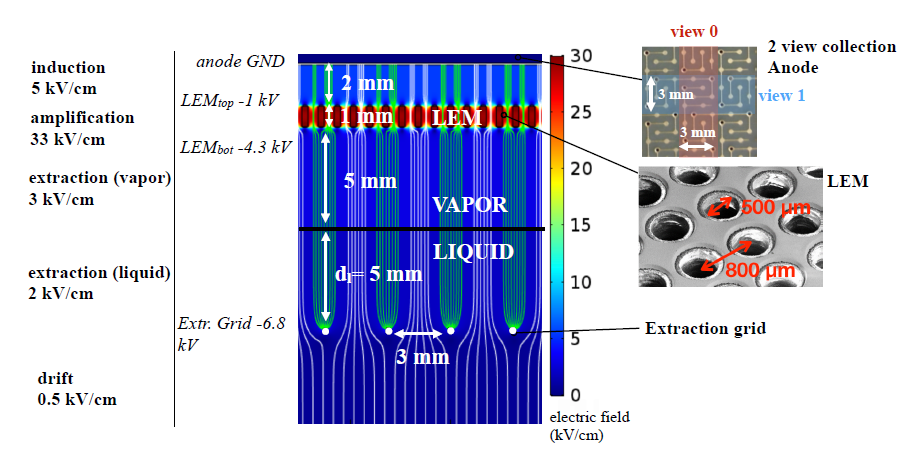
\includegraphics[width=.85\textwidth]{amplification-principle2}  
\end{dunefigure}
\begin{dunetable}[Interstage distances and \efield settings of the \dshort{dp} readout components]{lp{2cm}p{2cm}l}{tab:crp_dist}{Interstage distances and \efield settings of the \dword{dp} readout components.} 
 Component & Distance [mm] & Tolerance [mm] & \efield [kV/cm]  \\ \toprowrule
 Anode-\dword{lem} top electrode  & \num{2} & \num{0.1} & \numrange{2.5}{5}\\ \colhline
 \dword{lem} top-bottom electrode   & \num{1} & \num{0.01} & \numrange{30}{35}\\ \colhline
 \dword{lem} bottom electrode-grid        &\num{10} & \num{1} & \num{2} (in \lar) and \num{3} (in gaseous argon)\\
 \end{dunetable}

The extraction grid, the \num{36} \dwords{lem} and anodes composing a \dword{crp}, are assembled into a three-layered configuration of an area \SI{3}{\m}$\times$\SI{3}{\m} with precisely defined inter-stage distances and inter-alignment. Table~\ref{tab:crp_dist} shows the inter-stage distance and the tolerances required to obtain uniformity of gain to within $\sim$10\% at a LEM field of about \SI{31}kV/cm.
The anodes are connected horizontally in both the $x$ and $y$ directions to provide continuous \SI{3}{\m} long strips to be readout by the charge readout system described in Chapter~\ref{ch:dp-tpcelec}. Figure~\ref{fig:figure-label-crp} shows a general engineering view of a  fully assembled \dword{crp} and a photograph of a real one built in \num{2018} for \dword{pddp}.

\begin{dunefigure}
[View of a complete  $\SI{9}{m^{2}}$ CRP module]
{fig:figure-label-crp}
{Design view (left) of a complete assembled \dword{dp} $\SI{9}{m^{2}}$ \dword{crp} and real view (right) of one of the \dword{crp} built for \dword{pddp} just before being raised in the cryostat.}
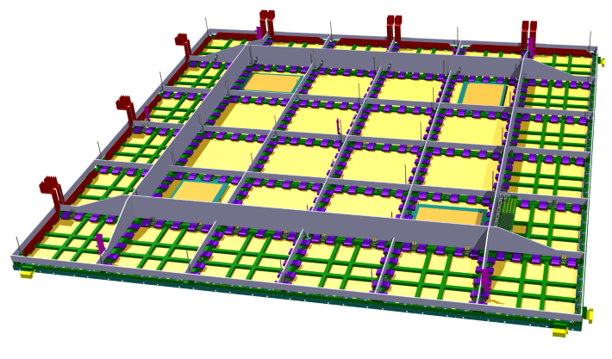
\includegraphics[width=0.48\textwidth]{CRP-fig1}
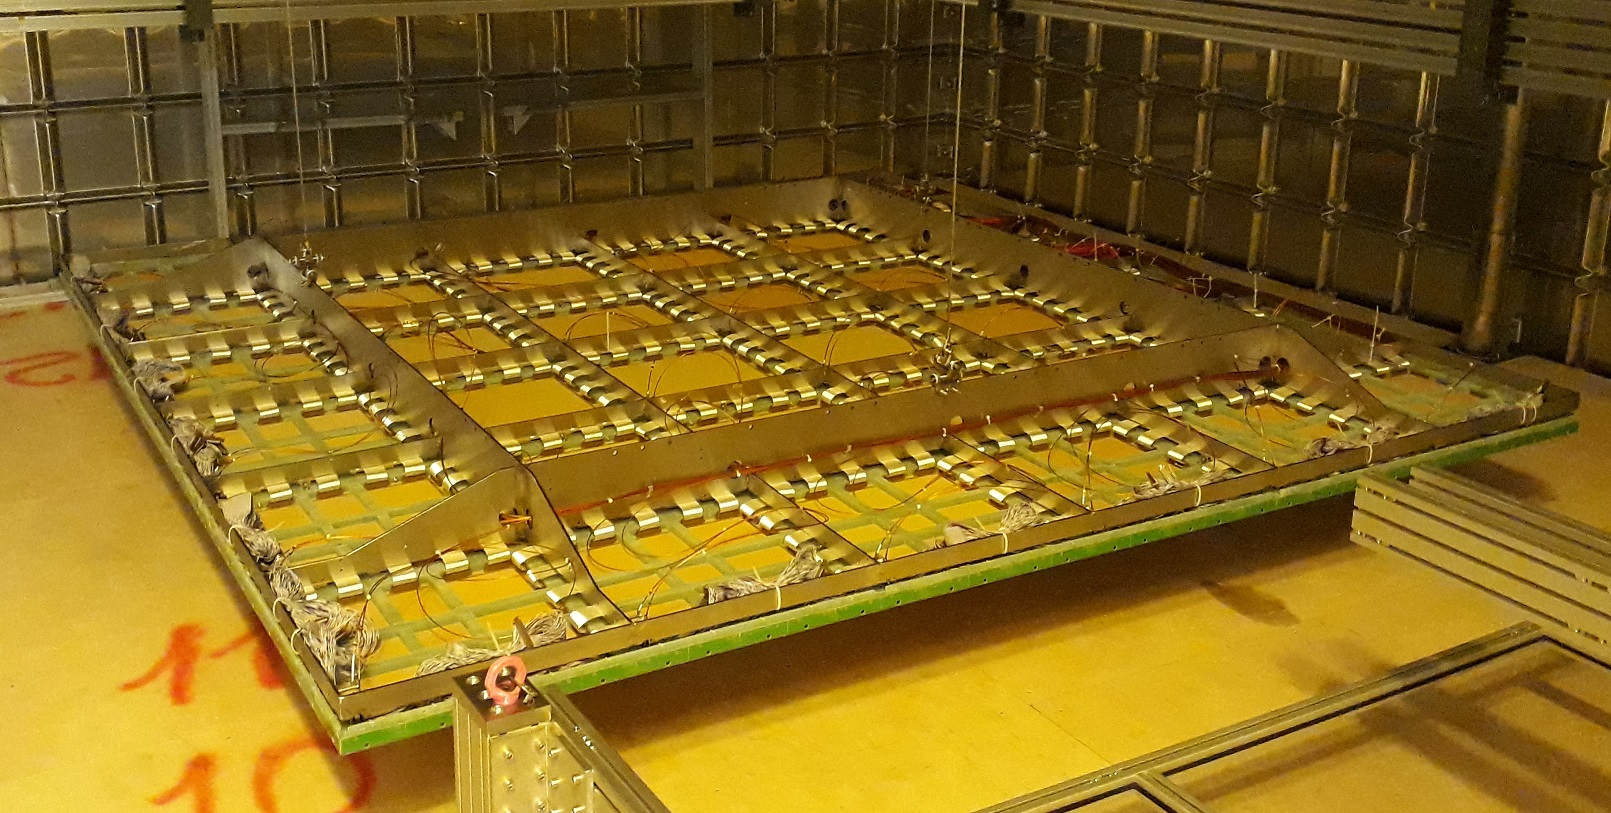
\includegraphics[width=0.50\textwidth]{CRP2-incryostatredim}
\end{dunefigure}

 

%%%%%%%%%%%%%%%%%%%%%%%%%%%%%%%%%%%%%%%%%%%%%%%
\subsection{Design Considerations and Requirements}
\label{ch:dp-crp-consider-requirements}

Each \dword{crp} is an independent detector element that performs charge extraction, multiplication, and collection and has its own \dword{hv} system and independent signal \fdth{}s. The entire area of the \dword{lem} and anode in a \dword{crp} is active. The positioning and the parallelism with the \dword{lar} surface can be individually adjusted for each \dword{crp}.

Figure~\ref{fig:figure-label-crp} shows the \dword{crp} mechanical structure that integrates the extraction grid and the \dword{lem}-anode system over a large area by minimizing dead space. The planarity of the active surface must be guaranteed despite possible sagging due to the three hanging points, the effects of differential thermal contraction on the various  components, and the presence of a temperature gradient in the gas phase, which could induce different thermal contractions as a function of distance from the liquid surface. To ensure planarity, the design  incorporates a support frame built of Invar, which can provide a stiff supporting structure extending vertically into the gas phase, with little sagging and very little contraction. The \dword{lem} and anodes, which would be affected by any significant thermal contraction, are integrated into a G10 planar structure with similar contraction properties. The G10 structure is mechanically decoupled from the Invar structure on the horizontal plane and is free to slide during thermal contraction.

The \dword{lem} and corresponding anode are mounted into 
\num{50}$\times$\SI{50}{cm$^2$}  
\dwords{las} on the \dword{crp} G10 mechanical supporting frame before assembly of the extraction grid. Each anode in a \dword{las} is segmented in \SI{50}{cm} long $x$ and $y$ strips. Adjacent \dword{las} anodes bridge together to form readout strips of the required length by connecting short flat cables to KEL\footnote{KEL 8925E-068-1795 .27mm Pitch, 2 piece, IDC for 0.635mm FC Connector, Low profile type, KEL Corporation\texttrademark{}, \url{https://www.kel.jp/english/product/}.} connectors soldered onto the top sides of the anodes. The signals from the last anode in each  strip chain are brought to \fdth{}s mounted on the other side of the front-end electronics embedded inside dedicated signal \fdth chimneys using \SI{120}{cm}-long flat cables.

Each \dword{crp} is independently hung from the vessel deck through its three suspension \fdth{}s. Each has its own \dword{hv} system, independent signal, and slow-control \fdth{}s.

Table~\ref{tab:specs:DP-CRP} summarizes the important specifications for \dword{dpmod} and parameters for the \dwords{crp} design. 
% This file is generated, any edits may be lost.

\begin{longtable}{p{0.14\textwidth}p{0.13\textwidth}p{0.18\textwidth}p{0.22\textwidth}p{0.20\textwidth}}
\caption{Specifications for DP-CRP \fixmehl{ref \texttt{tab:spec:DP-CRP}}} \\
  \rowcolor{dunesky}
       Label & Description  & Specification \newline (Goal) & Rationale & Validation \\  \colhline

   \newtag{DP-FD-1}{ spec:dp-min-drift-field }  & Minimum drift field  &  $>$\,\SI{250}{V/cm} \newline ( $>\,\SI{500}{V/cm}$ ) &  Lessens impacts of $e^-$-Ar recombination, $e^-$ lifetime, $e^-$ diffusion and space charge. &  ProtoDUNE \\ \colhline
    
   
  \newtag{DP-FD-2}{ spec:dp-system-noise }  & System noise  &  $<\,\SI{1000}\,e^-$ &  Studies suggest that a minimum of 5:1 S/N on individual strip measurements allows for sufficient reconstruction performance. &  ProtoDUNE and simulation \\ \colhline
    
   
  \newtag{DP-FD-3}{ spec:dp-light-yield }  & Light yield  &  $>\,\SI{1}{PE/MeV}$ (at anode), $>\,\SI{5}{PE/MeV}$ (avg  over active volume) &  Enable drift position determination of \dshort{ndk} candidates. Enable \dshort{pds}-based triggering on galactic SNBs. &  Full sim/reco of \dshort{ndk}, \dshort{snb} $\nu$ and radiological events. \\ \colhline
    
   \newtag{DP-FD-4}{ spec:time-resolution-pds }  & Time resolution  &  $<\,\SI{1}{\micro\second}$ \newline ( $<\,\SI{100}{\nano\second}$ ) &  Enables \SI{1}{mm} position resolution for \SI{10}{MeV} SNB candidate events for instantaneous rate $<\,\SI{1}{m^{-3}ms^{-1}}$. &   \\ \colhline
    
   \newtag{DP-FD-5}{ spec:lar-purity }  & Liquid argon purity  &  $<$\,\SI{100}{ppt} \newline ($<\,\SI{30}{ppt}$) &  Provides $>$5:1 S/N on induction planes for  pattern recognition and two-track separation. &  Purity monitors and cosmic ray tracks \\ \colhline
    
   \newtag{DP-FD-6}{ spec:crp-gaps }  & Gaps between CRPs   &  $<\,\SI{30}{mm}$ between adjacent CRPs \newline (\SI{6}{mm} (achieved among groups of adjacent CRPs)) &   &   \\ \colhline
    
   \newtag{DP-FD-8}{ spec:crp-eff-gain }  & CRP effective gain  &  \num{6} \newline (E.g., $\sim\,\num{20}$) &   &   \\ \colhline
    
   
  \newtag{DP-FD-9}{ spec:dp-crp-strip-spacing }  & CRP strips spacing  &  $<\,\SI{4.7}{mm}$ &  Enables 100\% efficient MIP detection, \SI{1.5}{cm} $yz$ vertex resolution. &  Simulation \\ \colhline
    
   
  \newtag{DP-FD-10}{ spec:crp-planarity }  & CRP planarity  &  $\pm\,\SI{0.75}{mm}$ &   &   \\ \colhline
    

   
  \newtag{DP-CRP-1}{ spec:crp-vert-precision }  & CRP vertical positioning precision  &  $<\,\SI{1}{\milli\meter}$ &  The extraction grid  must remain below the liquid argon surface &  Obtained by design \\ \colhline
    


\label{tab:specs:DP-CRP}
\end{longtable}


The main requirements for the \dwords{crp} concern their geometrical tolerances and their positioning with respect to the \dword{lar} level, so the extraction grid stays in the liquid while the bottom \dword{lem}'s surface is approximately \SI{5}{\mm} above the liquid surface. The requirements are:
\begin{itemize}
\item{ The \dword{crp} planarity should be well controlled over the \num{3}$\times$\SI{3}{\m^{2}} surface to guarantee the uniformity  of  the extraction field and the complete immersion of the extraction grid in \dword{lar}.  The ideal positioning of the 
extraction grid is \SI{5}{\mm} below the \dword{lar} surface. A planarity less than $\pm$\SI{0.75}{\mm}, obtained at  warm temperature, maintains the uniformity within $\pm$\SI{1}{\mm} according to simulations and \dword{pddp} experience during the \dword{crp} \coldbox tests. } 

\item{The precision of the \dword{crp} vertical positioning with the automated system should allow us to keep the extraction grid below the liquid surface at all times over the entire \dword{crp} area. It should not add more  than  \SI{1}{\mm} to the planarity tolerance discussed above. The automated system drive guarantees a position precision of more than \SI{0.1}{\mm} on the \dword{crp} height, and the capacitive measurements of the liquid level should allow regulating the height with precision of more than  \num{250}$\mu$m}.

\item{Lateral inter-\dword{crp} dead space should be maintained at values  
< \SI{30}{mm}.
Allowing gaps between \dwords{crp} is mandatory for positioning the \dword{crp} and to install the grid supports along the edges of the active \dword{crp} surface. This also simplifies detector construction and installation. The \dword{pddp} installation shows that a maximum distance of  \SI{6}{\mm}  is already achieved. 
For \dword{dune} \dword{dpmod}, gaps up to \SI{30}{\mm} may  exist between some groups of \dwords{crp}, allowing adjustments for thermal shrinkage over the whole  \num{60}$\times$\SI{12}{\m^{2}} readout area.}

\item{The equivalent S/N ratio of \num{6.6} can be achieved for signals coming from the extreme end of the \SI{12}{\m} drift. This assumes an electron lifetime corresponding to  the minimal requirement of \SI{5}{\ms} with a noise level of \num{1000} electrons, a minimal  effective \dword{crp} gain of \num{6}, and a minimal drift field of \SI{250}{V/cm}. This figure translates for \SI{5}{\ms} electron lifetime into a S/N ratio of  \num{20} for \SI{6}{\m} drift and \num{34.6} for \SI{3}{\m} drift. }

\item{With a \SI{4.7}{\mm} pitch between the anode strips, the S/N is consistent with 100\% hit reconstruction efficiency for  \dwords{mip} and provides \SI{1.5}{cm} vertex resolution in $y-z$ plane.
The present  design of the anode and \dword{lem} has already achieved \SI{3.125}{\mm}}.
\end{itemize}
The \dword{crp} design for the \dword{dpmod} is based on the one developed for \dword{pddp} with the exact same dimensions and 
the same requirements.
%%%%%%%%%%%%%%%%%%%%%%%%%%%%%%%%%%%%%%%%%%%%%%
\subsection{Scope}
\label{ch:dp-crp-scope}

The scope of the \dword{crp} system, provided by the \dword{crp} consortium, covers the procurement of materials, fabrication, testing, delivery, and installation of all components needed to complete the \dword{crp} array for a \dword{dune} \dword{dpmod}{}. It includes the following systems: 
\begin{itemize}
\item  Production and \dword{qa} of the \dword{lem} and anodes;
\item  Production of the G10 and Invar frames;
\item Production of the suspension \fdth{}s and motorization;
\item Production of the extraction grid elements;
\item Production of the \dword{hv} distribution system associated with the \dword{crp} for applying voltages to the \dword{lem} and grid;
\item Production of the temperature probe system associated with the \dword{crp};
\item Production of the level meter system associated with the \dword{crp};
\item Production of the anode strips pulsing system  
associated with the \dwords{crp};
\item Production of the transportation and storage boxes for the \dwords{crp};
\item Assembly of the \dword{crp} structures, \dword{las}, extraction grid elements, \dword{hv}, slow controls, and cabling for each \dword{crp};
\item Testing of the assembled \dwords{crp};
\item Packing these \dwords{crp} into storage boxes;
\item Placing the \dwords{crp} into transport boxes and delivering them to \dword{surf}{}; 
\item \coldbox tests of the \dwords{crp} underground;
\item Installing, cabling, and testing the \dwords{crp} in the cryostat.
\end{itemize}

%%%%%%%%%%%%%%%%%%%%%%%%%%%%%%%%%%%%%%%%%%%%%%%%
\section{CRP Design}
\label{ch:dp-crp-design}
The design described in this section is primarily based on the one developed for \dword{dpmod}. The scaling to \dword{dune} \dword{dpmod} is straightforward because the \dword{crp} unit is identical in its dimensions, high voltage conditions, and instrumentation. Some upgrades may be needed after constructing and installing the \dword{pddp} and running the detector.

A complete \dword{crp} system includes, as illustrated in Figure~\ref{fig:figure-label-crp2}:
\begin{itemize}
\item Mechanical frames (Invar and G10) and decoupling system,
\item Detection plane made of \dwords{lem} and anodes,
\item Extraction grid,
\item Instrumentation devices: level meters, distance meters, and temperature probes,
\item Internal cabling: to patch panels (\dword{lem} \dword{hv}, slow control instruments),
\item Suspension and control system.
\end{itemize}

\begin{dunefigure}[Main components of a CRP module of  \SI{9}{m$^{2}$}]{fig:figure-label-crp2}
{Main components of a \dword{crp} module of  \SI{9}{m$^{2}$}.}
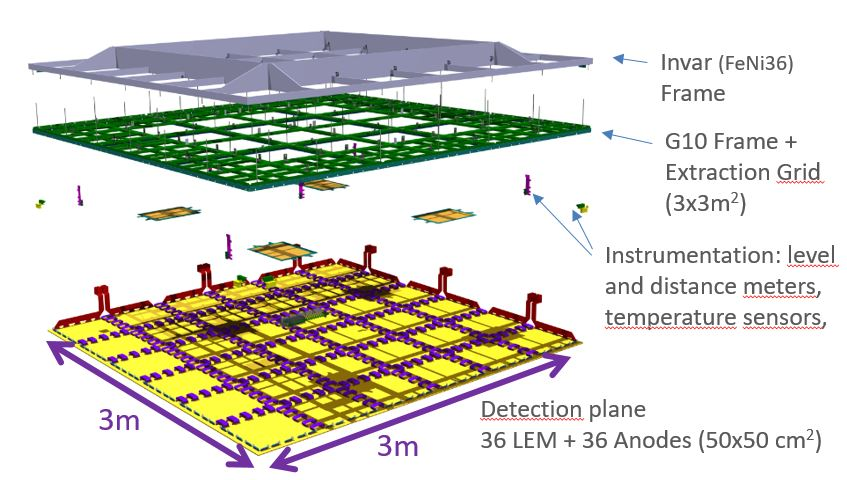
\includegraphics[width=0.8\textwidth]{CRP-design-components}
\end{dunefigure}

%%%%%%%%%%%%%%%%%%%%%%%%%%%%%%%%%%%
\subsection{Mechanical Structure}
\label{sec:fddp-crp-mechanics}
%%%%%%%%%%%%%%%%%%%
\subsubsection{Invar Frame}

The main mechanical supporting structure of the \dword{crp} is made of Invar, a nickel-iron alloy. This material was chosen for its low coefficient of thermal expansion leading to very little deformation at cold temperatures, especially in the argon gas where the temperature gradient in the cryostat may be a few \si{K/cm}. 
The thermal contraction coefficient of Invar (alpha =  1.5 10-6 K-1) is 10 times less than the ones of stainless steel.  Considering a temperature, change of nearly 200 degrees from ambient to the liquid argon temperature the thermal shrinkage of the Invar frame along the 3m sides is less than 1mm.  With the vertical temperature gradient of about 2 K/cm  expected along the vertical dimension (250mm)  the difference between the bottom and the top of the Invar beam will generate a maximal vertical deformation less than 0.3mm at its highest point. In case of a stainless steel structure the deformation is more than 2mm over 3m length beams which is above the requirement of planarity. Those results have been obtained from measurements in cold bath and found compatible with the FEA calculations used for the \dword{crp} design.
The structure consists of a grid of soldered Invar beams \SI{3000}{mm} long and \SI{6.5}{mm} wide. The four main beams are \SI{150}{mm} high while the internal beams are \SI{40}{mm} high, as are the four surrounding plates. The heights have been optimized to keep the necessary stiffness and reduce the total frame weight to approximately \SI{112}{kg}.
 Figure~\ref{fig:invarframe} shows the construction of one of the first \dword{crp} frames for \dword{pddp} at the company.
\begin{dunefigure}[First CRP Invar frame under construction for ProtoDUNE-DP]{fig:invarframe}
{First \dword{crp} Invar frame under construction for \dword{pddp}}
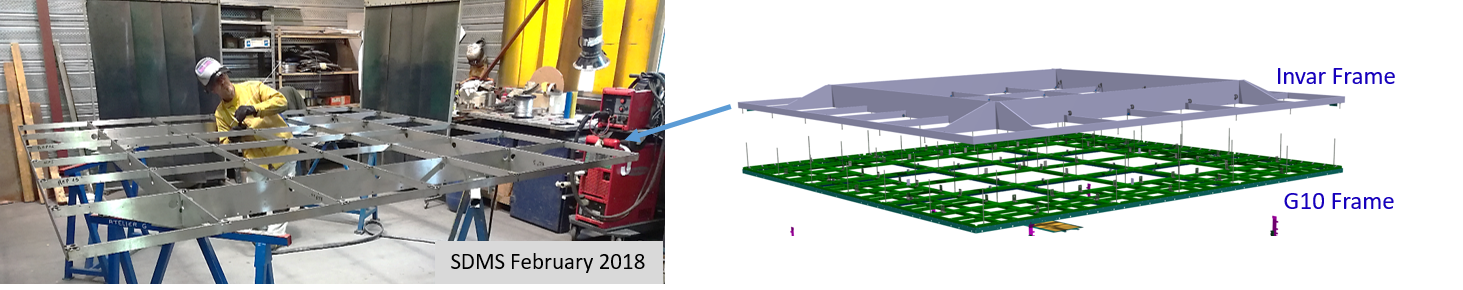
\includegraphics[width=0.95\textwidth]{invar-framev2}
\end{dunefigure}
 \subsubsection{G10 Frames and Modules}
\label{sec:invar-frame}

The \num{3}$\times$\SI{3}{m$^{2}$}  G10 fiberglass structure used to attach the \num{36} \dwords{lem} and anodes, the extraction grid, and level meters comprise nine \num{1}$\times$\SI{1}{m$^{2}$} subframes. The choice of G10 is driven by the need to match the \dword{lem} and anode thermo-mechanical behavior and avoid over-stress due to differential thermal contraction. 
Figure~\ref{fig:crp-g10} shows the pattern of the nine G10 parts composing a full \dword{crp} frame, the supporting comb positioned every meter, and the extraction grid support plates along the side of the \dword{crp}. The picture on the right shows a G10 frame built for a \dword{pddp} \dword{crp}.

\begin{dunefigure}[G10 elements of a full CRP module]{fig:crp-g10}
{G10 elements of a full \dword{crp} module}
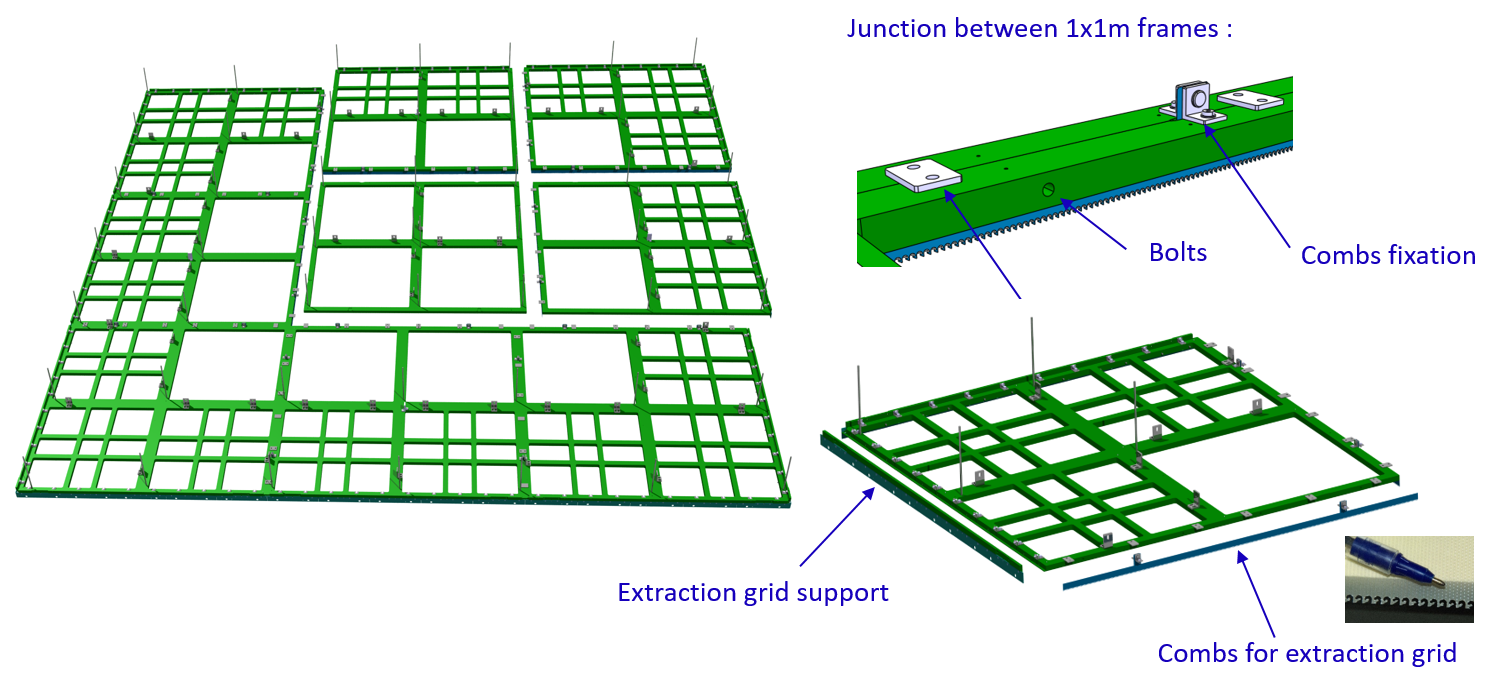
\includegraphics[width=0.63\textwidth]{G10}
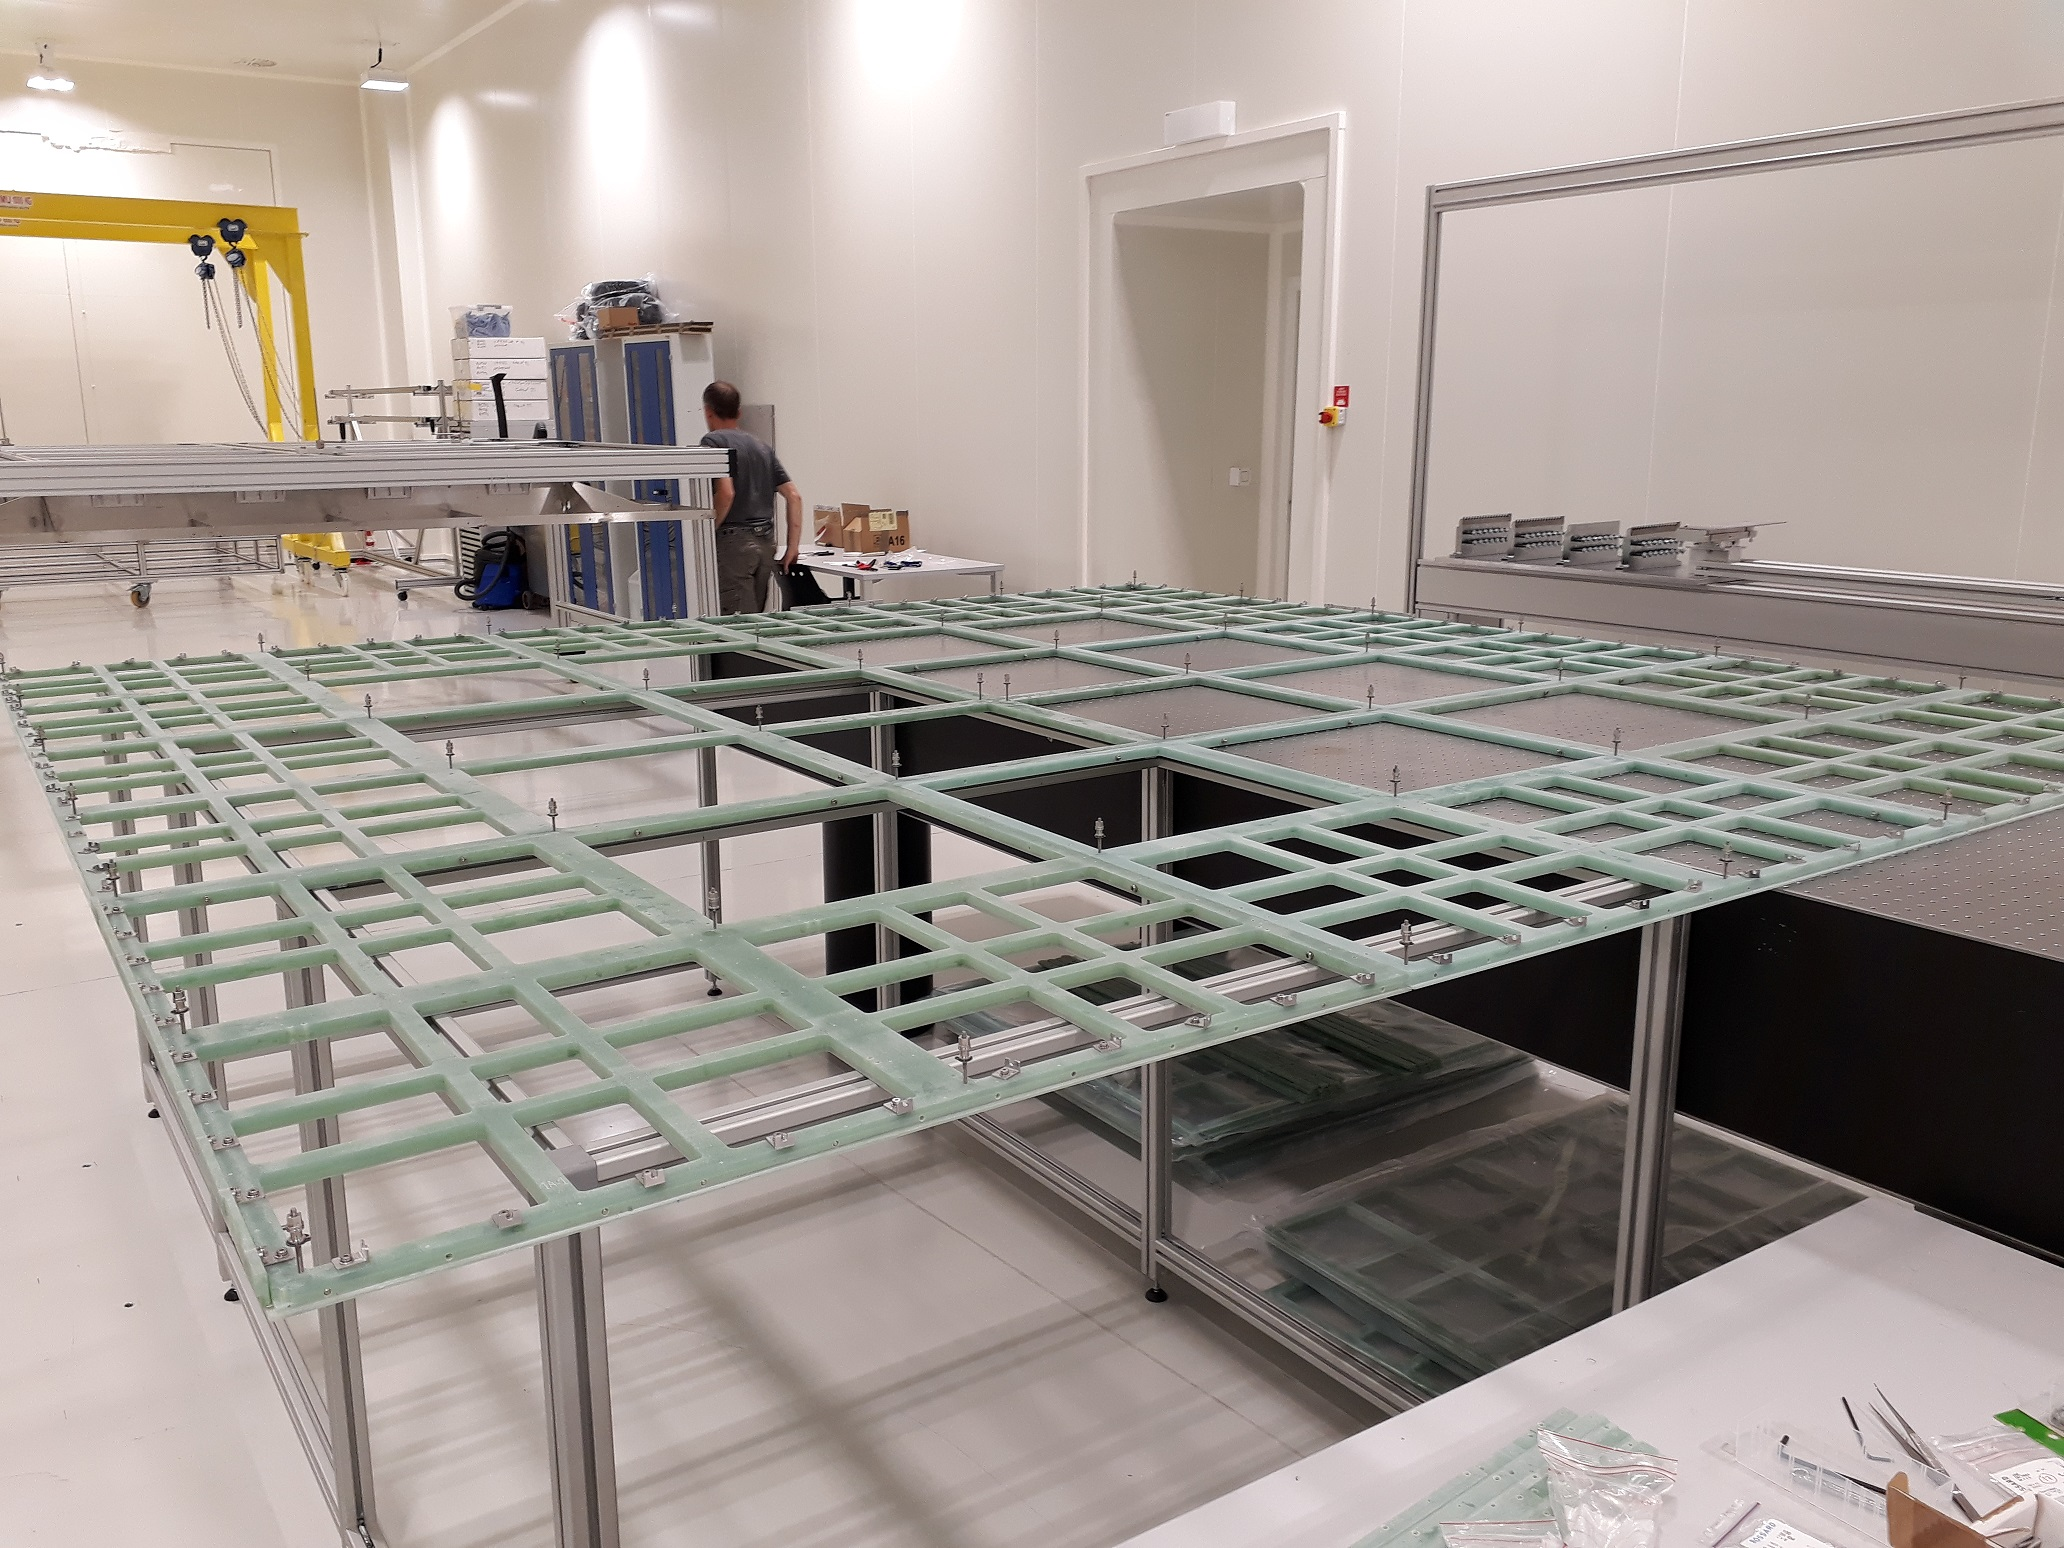
\includegraphics[width=0.36\textwidth]{G10-frameassembled}
\end{dunefigure}

Because G10 is a composite material created by stacking multiple layers of glass fibers, the orientation of the stacking must be considered before assembly.
At the construction level, the fiber directions are matched between the different subframes to ensure homogeneity in thermal shrinkage. Three different patterns must be produced, one for the four angles, one for the four face centers, and one for the central subframe. This assembly procedure is supported by detailed FEA calculations.
Two versions of each pattern for the supporting extraction grid bars and the combs follow the same rule.

The subframes have been designed to guarantee  
adequate stiffness in the  regions subject to more tension while minimizing material to reduce weight.
The G10 structure is \SI{15}{mm} thick and weighs approximately \SI{68}{kg}. 

\subsubsection{Decoupling System}
 
During cooling, Invar's dimensions remain nearly unchanged while the G10 frame and \dwords{lem}-anodes contract similarly. Thermal decoupling allows a lateral sliding of the G10 frame without changing the level. 
Dedicated decoupling systems are installed at each corner of the Invar frame (\num{50} systems by  \num{3}$\times$\SI{3}{m$^{2}$} module). One decoupling system that allows the G10 and \dword{lem}-anode elements to slide is shown in  Figure~\ref{fig:crp-decoupling}.

\begin{dunefigure}[Decoupling system attached to the Invar frame]{fig:crp-decoupling}
{Decoupling system attached to the Invar frame, detailed view. Example of one system built for \dword{pddp} and one decoupling system attached to the Invar frame of a \dword{crp}.}
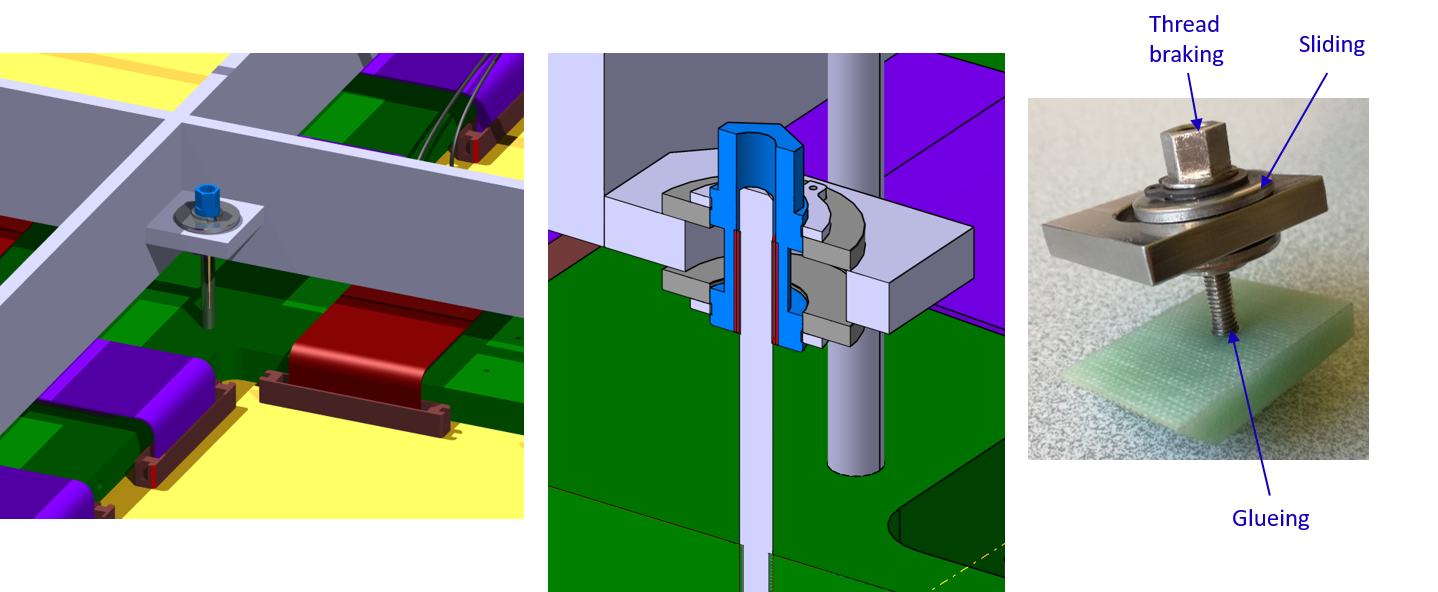
\includegraphics[width=0.68\textwidth]{decoupling}
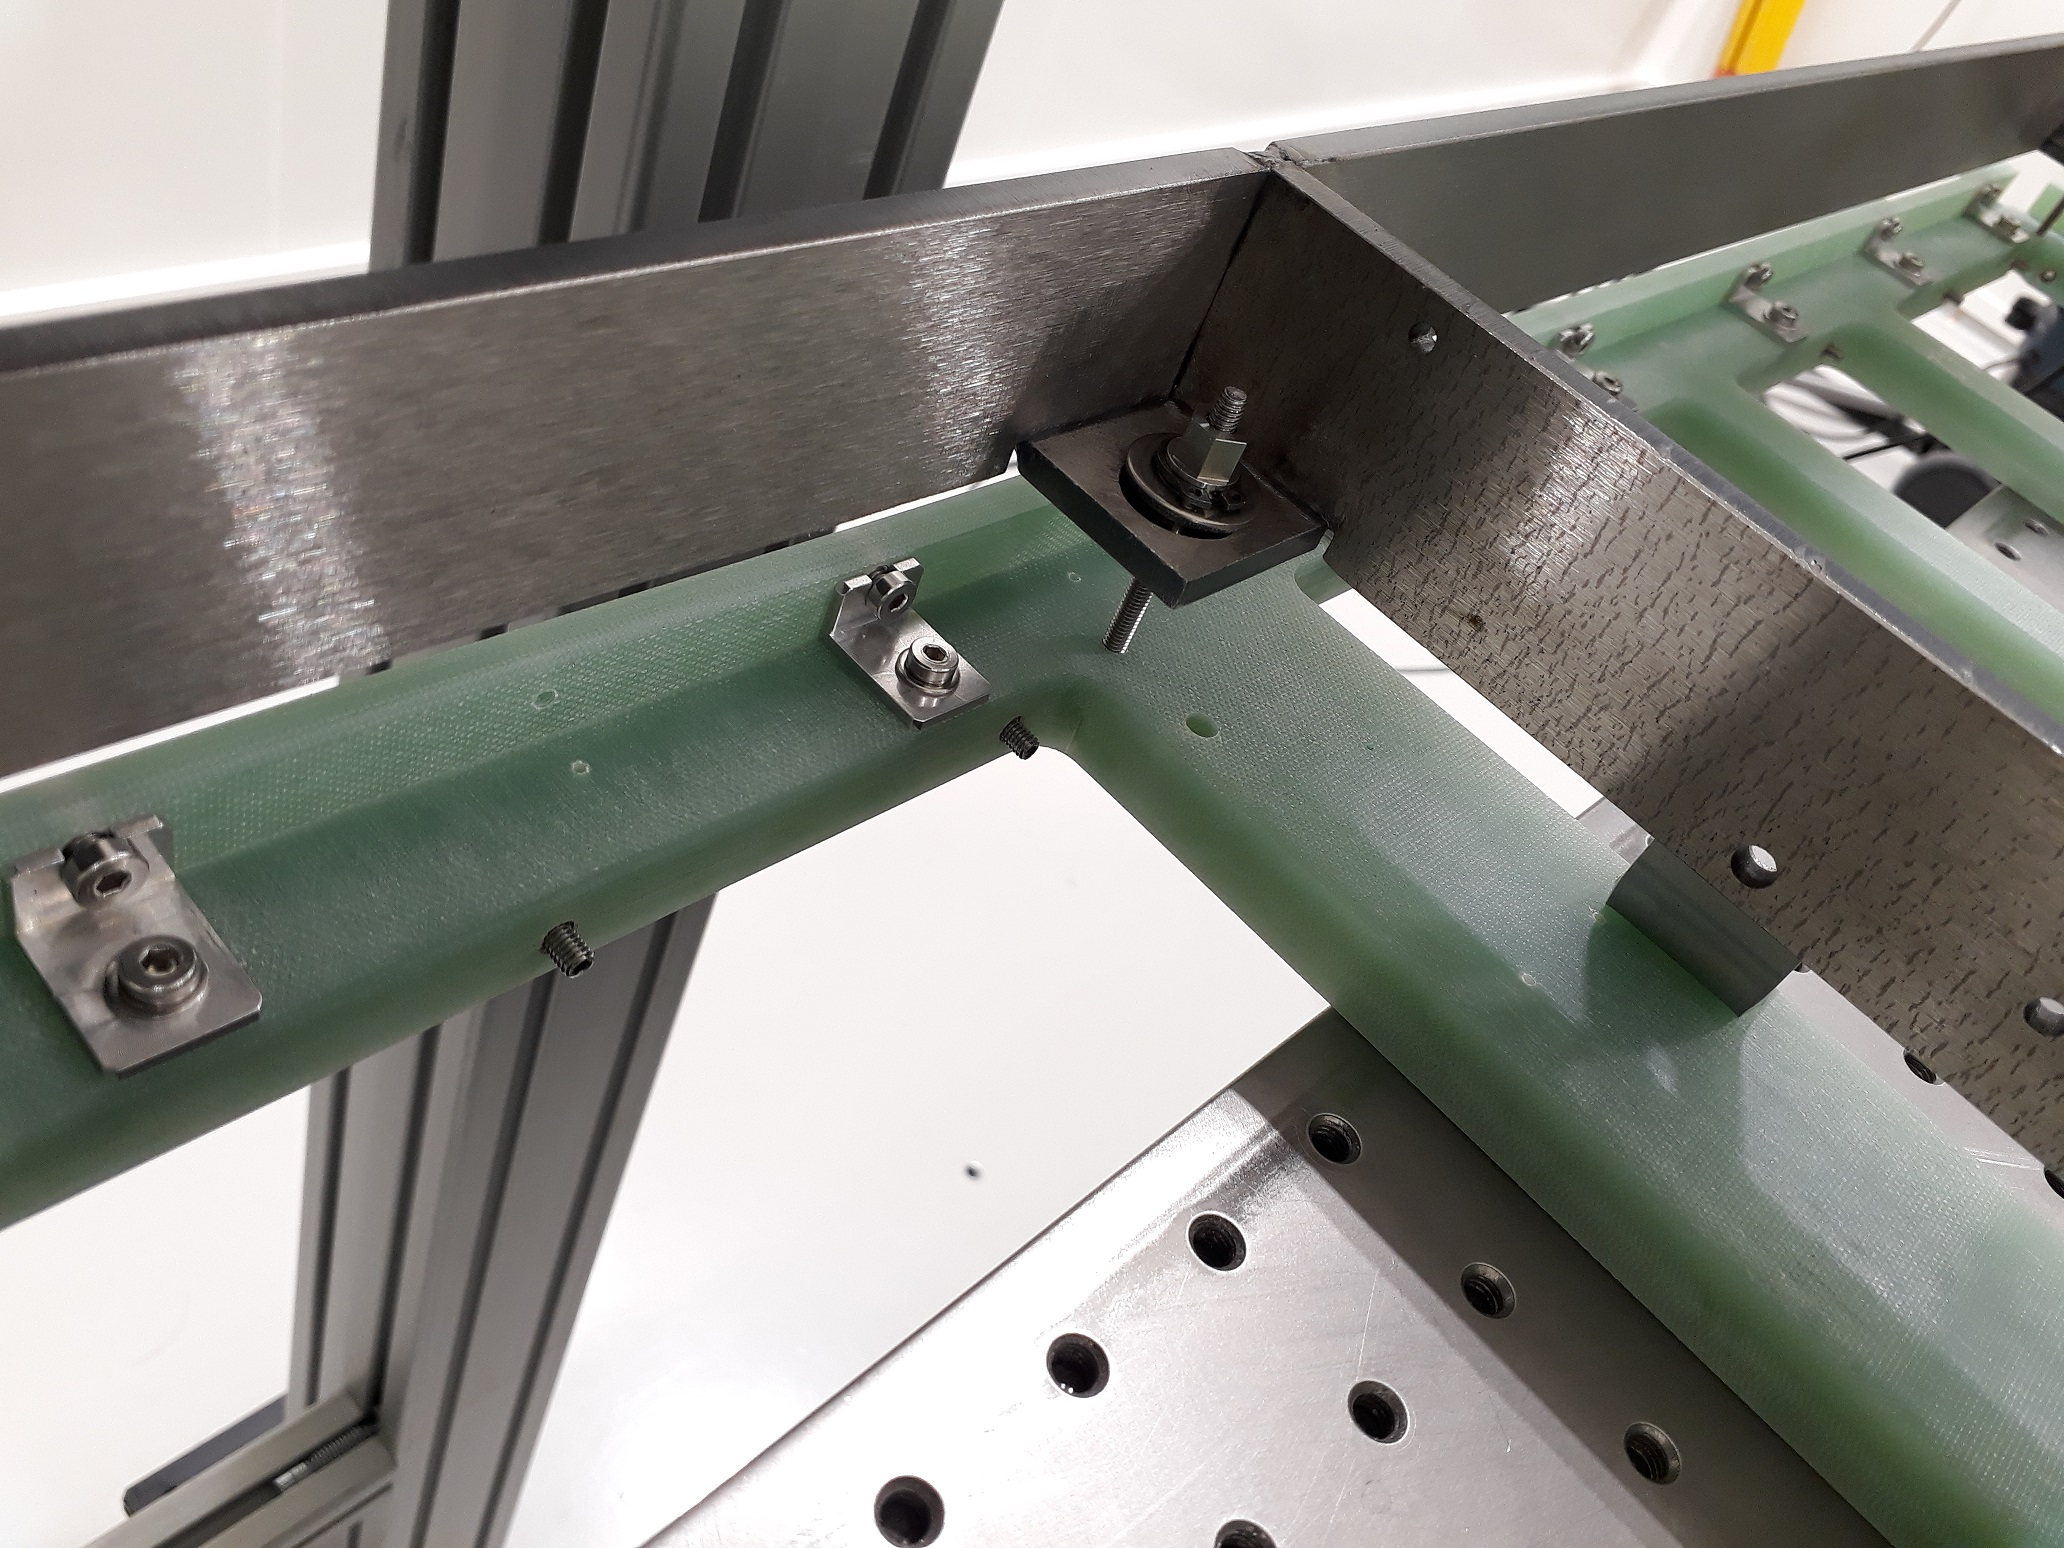
\includegraphics[width=0.30\textwidth]{decoupling-crp}
\end{dunefigure}

The total weight of a \dword{crp} including \dwords{lem} and anodes is approximately \SI{330}{kg}.

%%%%%%%%%%%%%%%%%%%%%%%%%%%%%%%%%%%
\subsection{Extraction Grid}
\label{sec:fddp-crp-grid}
The extraction grid consists of \SI{100}{\micro\meter}-diameter stainless steel wires tensioned in both $x$ and $y$ directions over the entire \SI{3}{m} length and width of the \dword{crp} with a \dpstrippitch pitch. They are soldered into groups of \num{64} on independent wire-tensioning pads perpendicular to the side of the \dword{crp} frame. Each wire-tensioning pad consists of a \dword{pcb} \SI{1.6}{mm} wide and \SI{20}{cm} long that is fixed very precisely to mechanical support beams screwed to the G10 frame of the \dword{crp}, as shown in Figure~\ref{fig:grid-parts}.
\begin{dunefigure}[Extraction grid components on the CRP structure]{fig:grid-parts}
{Extraction grid components on the \dword{crp} structure. On the left are the \dword{pcb} plates and their supporting bars. On the right is the  
wire tensioning system with the pushing screws and calibrated wedges to keep the right distance.}
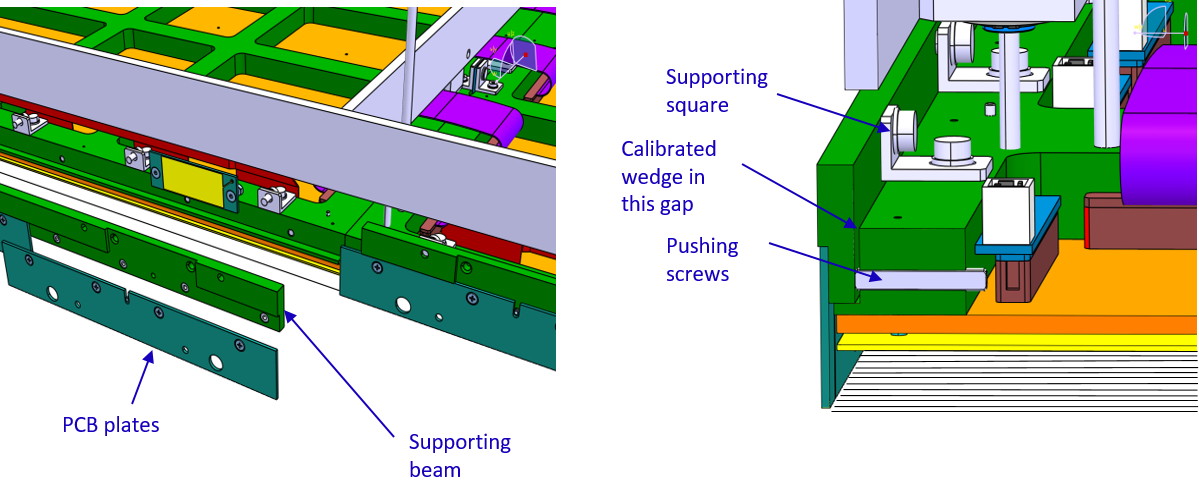
\includegraphics[width=0.8\textwidth]{grid-parts}
\end{dunefigure}

The \dword{pcb} has \num{64} soldering pads with \SI{200}{\micro\meter} grooves for precise positioning of the wires. During the 
soldering process, each wire is tensioned and positioned in a groove. The \dword{pcb} is then mounted on the G10 supporting bars, and the tension of the group of \num{64} wires can be precisely adjusted by pushing the supporting bars against the \dword{crp}'s G10 frame with screws. The tensioning is performed by tightening pushing screws, adding a calibrated wedge, and locking the supporting square.
Supporting the comb-teeth blades inserted between the \SI{1}{m$^2$} G10 subframes in both $x$ and $y$ directions restricts any sag in the wires to \SI{0.1}{mm}, which are \SI{3}{m} long in both directions. The array of blades penetrates the liquid surface and has the additional benefit of acting as a baffle against potential surface waves in the \dword{lar}.

The grid \dword{hv} connection for a \dword{crp} is made through a varnished copper track into one of the \dword{crp}'s \num{60} \dword{pcb} plates; a special isolated connection  is made inside the \dword{crp} structure.

%%%%%%%%%%%%%%%%%%%%%%%%%%%%%%%%%%%
\subsection{Large Electron Multiplier (LEM)}
\label{sec:fddp-crp-lem}

Each \dword{lem} consists of a \SI{1}{mm}-thick,  \num{50}$\times$\SI{50}{cm$^{2}$} copper-clad standard \dword{pcb} epoxy plate. Holes \SI{500}{\micro\meter} in diameter, through which electrons undergo amplification, are mechanically drilled in a hexagonal pattern with a pitch of \SI{800}{\micro\meter}, yielding approximately \num{180} holes per \si{cm$^2$}. In addition, each hole has a  \SI{40}{\micro\meter} dielectric rim, obtained by a chemical process, to prevent electrical discharges from occurring near the holes. The holes confine the UV photons produced during the avalanche process and thus act as a mechanical quencher to prevent photon feedback. This property makes the \dword{lem} suitable for operation in ultra-pure argon vapor without adding a quenching gas. The final gold-plated copper thickness of each \dword{lem} electrode is approximately  \SI{60}{\micro\meter}. Twenty peripheral and nine central \SI{2.2}{mm}-diameter holes are used to assemble the \dword{lem}  to its anode on the G10 frame. Figure~\ref{fig:LEM_CFR-35} shows a picture of a \dword{lem} module used for  \dword{pddp}. To prevent \dword{hv} discharges near or across the edges, the \dword{lem} module has a  \SI{10}{mm} border free of metal and another \SI{5}{mm} copper guard ring. Similar copper guard rings are located around the \SI{2.2}{mm} diameter holes and the \dword{hv} connectors. The latter are made of \SI{1.2}{mm} diameter male pins (Deutsch\footnote{Deutsch\texttrademark{} \url{http://www.deutsch.net/}.} 6860-201-22278.) soldered onto specifically designed pads imprinted on the \dword{lem} electrodes. The pins are insulated with circular tubes made in MACOR with a \SI{10}{mm} circular clearance around each pin. 

The total active area of a \dword{lem} module used for  \dword{pddp} represents approximately \SI{86}{\%} of the \num{50}$\times$\SI{50}{cm$^{2}$} area. The choice of the \dword{lem} design for \dword{pddp} allows achieving stable operation conditions up to \SI{3.5}{kV} in \dword{dp} \dword{lar} mode, corresponding to amplification gains larger than \num{30} (\num{100}) after (before) charging up the \dword{lem} dielectric material. For the \dword{dpmod}, the current \dword{lem} design will be further optimized to find the best compromise between the detector active area and operation stability.

\begin{dunefigure}
[Picture of a LEM module used for ProtoDUNE-DP]
{fig:LEM_CFR-35}
{Picture of a \dword{lem} module used for  \dword{pddp}.}
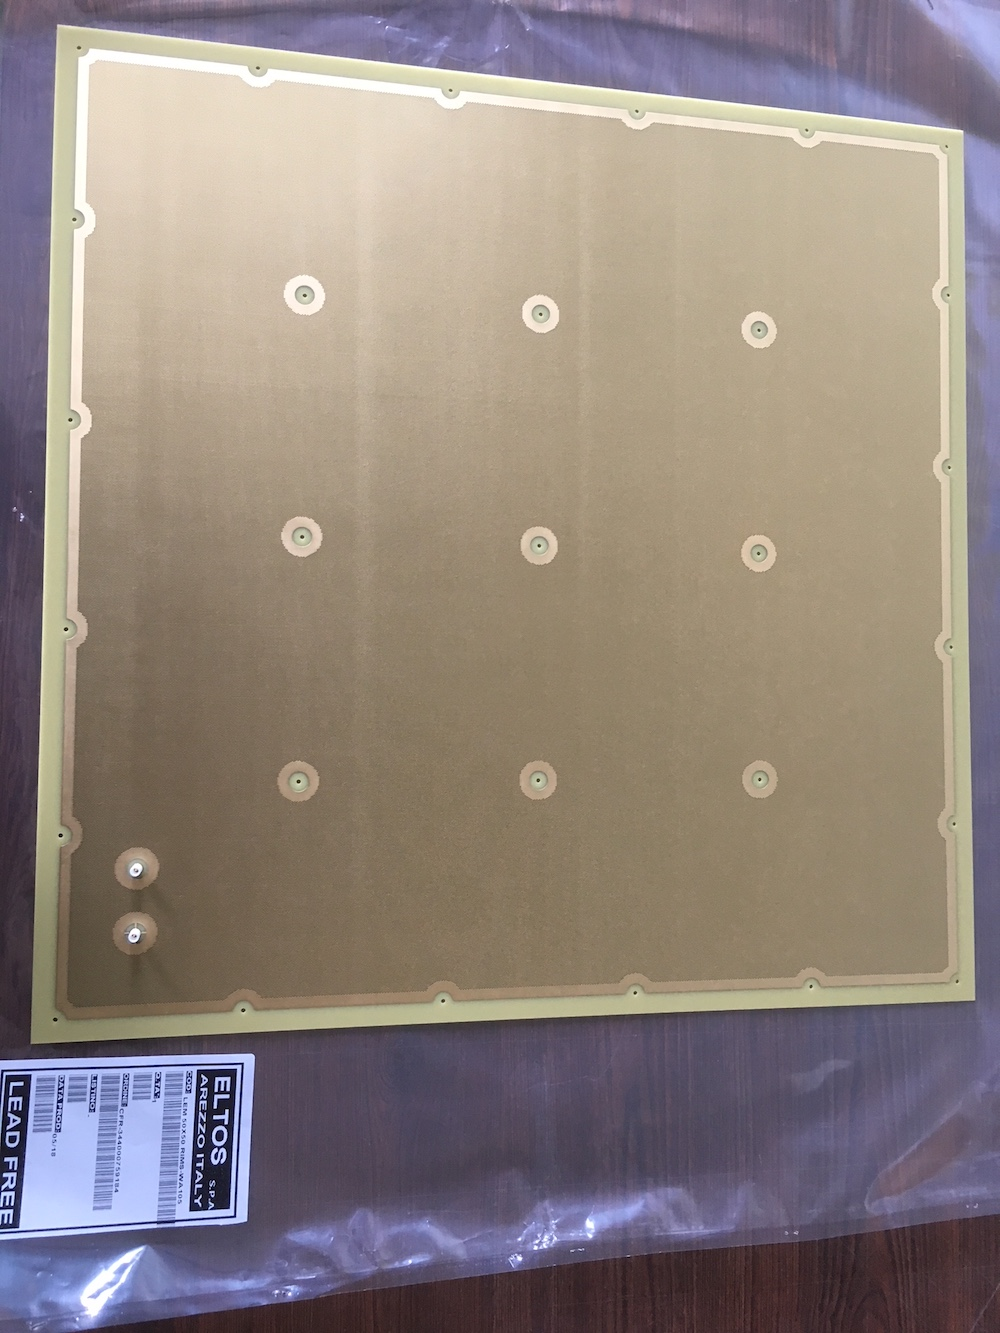
\includegraphics[width=.75\textwidth]{LEM_CFR-35}
\end{dunefigure}

%%%%%%%%%%%%%%%%%%%%%%%%%%%%%%%%%%%
\subsection{Anode}
\label{sec:fddp-crp-anode}
 
The anode is a four-layer \dword{pcb} with a set of orthogonal strips with a \dpstrippitch pitch that provide the two views of the collected charge. The area of the anode is the same as for the \dword{lem}:  \num{50}$\times$\SI{50}{cm$^2$}. Twenty nine holes \SI{2.2}{mm} in diameter matching the \dword{lem} holes are used for the \dword{lem} and anode assembly on their G10 frame. The \SI{2}{mm} distance between the anode and the \dword{lem} is ensured by \num{29} precisely machined spacers made of polyetheretherketone (PEEK). 

The pattern of readout strips, printed on the bottom \dword{pcb} layer and used for charge collection, is optimized to evenly split the charge between both views (Figure~\ref{fig:Anode}). Electrical insulation in the locations where orthogonal tracks would superimpose is achieved by 
using a system of vias between the top and bottom layers of the \dword{pcb} to allow the tracks to cross over and under one another. 
Each strip, made of thin gold-plated copper tracks, has a capacitance per unit length to ground of approximately 
\SI{160}{pF/m}. The readout strips are routed to the top layer towards \num{68}-pin female connectors (KEL 8925E-068-179-F) soldered on the anode periphery. Each connector reads \num{32} strips; its \num{36} remaining pins are connected to the detector ground via a copper strip that runs around the periphery of the top layer of the anode (see Figure \ref{fig:Anode}). 

\begin{dunefigure}
[Picture of the anode symmetric \twod strip design.]
{fig:Anode}
{Picture of the anode symmetric \twod strip design.}
  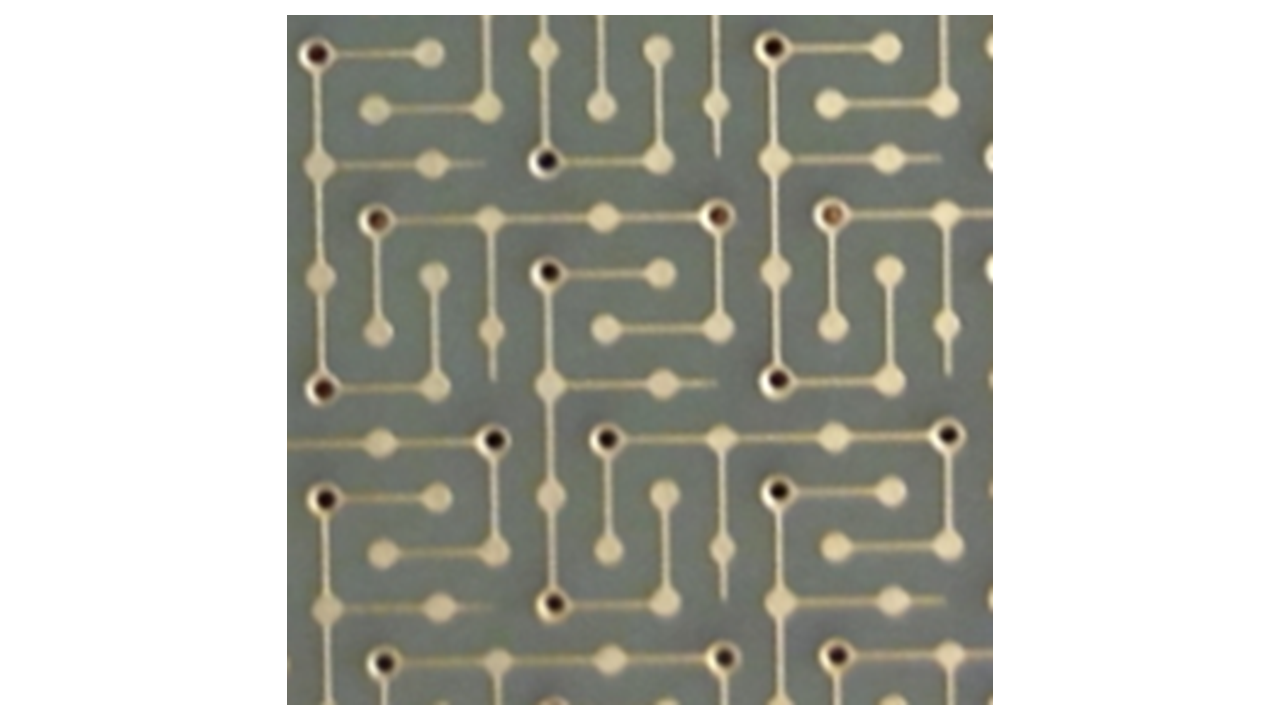
\includegraphics[width=.7\textwidth]{Anode_strips}
\end{dunefigure}

%%%%%%%%%%%%%%%%%%%%%%%%%%%%%%%%%%
\subsection{Instrumentation}
\label{sec:fddp-crp-instr}

\subsubsection{High Voltage distribution and cabling}

.... Division of LEM HV distribution

\subsubsection{Distance meters and level meters}

The vertical and lateral positions of the \dwords{crp} are measured using different instruments. 
The vertical position of the \dword{crp} can be determined both from the suspension system and from dedicated capacitive measurements.
The  suspension system and its motorization on three points provides an accurate measurement for each \dword{crp} within approximately \SI{0.1}{mm} because of the accuracy of the stepper motors and encoders. 
To set properly the reference position of the encoders the anchor points on the \dword{crp} must be surveyed during construction, and the absolute positions of the suspensions must be surveyed from the roof of the cryostat while the \fdth{}s are installed. These absolute positions of the suspension feedthroughs on the roof of the cryostat are surveyed with a precision of 0.5mm to get a reference position in all three dimensions. The finer relative calibration of the vertical positioning of the CRP is done from inside the cryostat after raising the CRP to their nominal positions. The relative vertical position survey is done with 0.1 mm accuracy and the encoders are then set according to the position found.

The position \dword{crp} relative to the \dword{lar} level can be measured using capacitive level meters on the sides of the \dwords{crp} located at the periphery of the  $\SI{60}{m}\times\SI{12}{m}$ detection plane.  The  measurements of the capacitance between the \dword{lem} and the extraction grid, which depend on the height of the liquid above the grid, can also provide a  measurement  of the \dword{crp}'s vertical position relative to the liquid surface. This method is used for the \dwords{crp} that are not located at the periphery, while the ones at the periphery can exploit both the  \dword{lem}-grid capacitance measurements and the capacitive level meters.
 
The distance between each \dword{crp} pair is measured using capacitive devices called distance meters made of two parallel electrode plates.  
This measurement allows the \dwords{crp} to be positioned with the correct  inter-\dword{crp} distance all along the detection plane. These devices do not require any contact with  \dwords{crp} and are accurate to within approximately \SI{0.1}{mm} on the  inter-\dword{crp} distance. The \dwords{crp} inter-distance should be known within \SI{0.5}{mm}.  Four devices per \dword{crp} side are embedded in the G10 frame side (see Figure~\ref{fig:distancemeter}).

\begin{dunefigure}[View of the distance meter plates on the sides of a CRP]{fig:distancemeter}
{CAD views (left, center) of the distance meter plates, represented by the yellow rectangles, on the sides of a \dword{crp}. Two different plate sizes are used in pairs, installed on facing sides of neighboring \dwords{crp}, 
to increase the measurement accuracy of the overlapping surface, which translates in the capacitance to be measured. Right: a photograph of a set of five distance meter plates of the two sizes received from the production factory.}
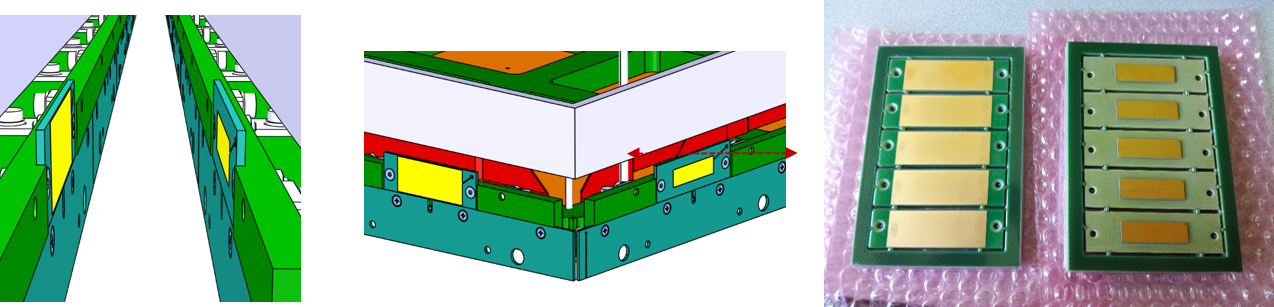
\includegraphics[width=0.85\textwidth]{distancemeter}
\end{dunefigure}

\subsubsection{Thermometers}

The temperature in the gas above the anode plane is monitored at different heights with resistance thermometers (Pt sensors) soldered on  six \dword{pcb} boards distributed over the full surface of the \dword{crp}, six 
sensors per \dword{pcb}. Figure~\ref{fig:ptsensor} shows the configuration and the Pt positions.

\begin{dunefigure}[View of the thermometer board]{fig:ptsensor}
{View of the thermometer board and the positions of the Pt sensors along the \dword{pcb} plate.}
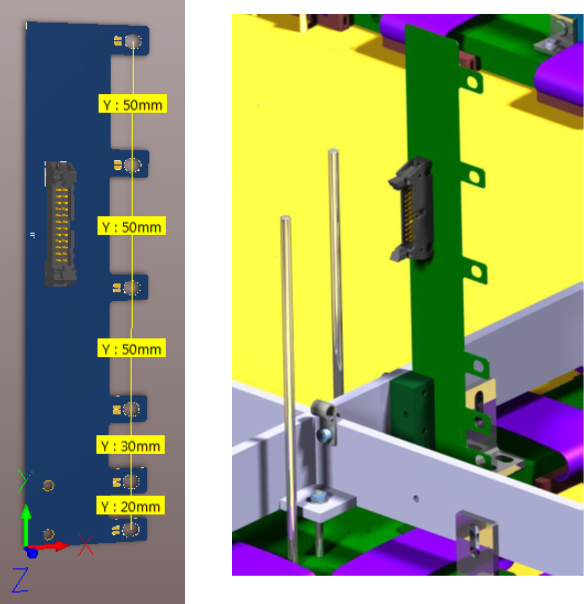
\includegraphics[width=0.45\textwidth]{ptsensor}
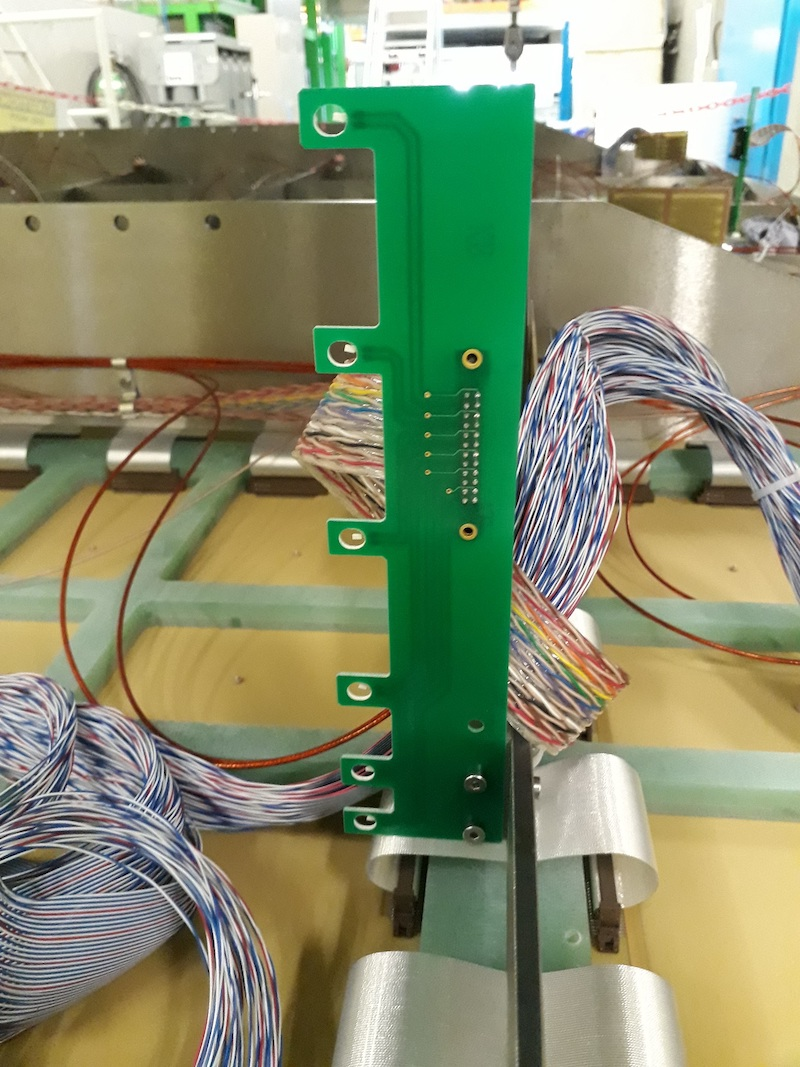
\includegraphics[width=0.34\textwidth]{ptsensor-crp}
\end{dunefigure}


%%%%%%%%%%%%%%%%%%%%%%%%%%%%%%%%%%%
\subsection{Suspension System and Drive}
\label{sec:fddp-crp-suspension}

Three suspension \fdth{}s are arranged in an equilateral triangle whose barycenter coincides with that of the \dword{crp}; an automated system is used to suspend the \dword{crp} at the required position and precisely adjust the \dword{crp} level with respect to the \dword{lar} surface.

Figure~\ref{fig:spft} shows the design of the suspension \fdth including the bellows and the motors to be installed on top of the cryostat. There are three \fdth{}s per \dword{crp}. The picture on the right shows one of the twelve suspension systems built and installed on the \dword{pddp} cryostat roof.

\begin{dunefigure}[Suspension \fdth and various assembly details]{fig:spft}
{Suspension \fdth and various assembly details. The picture on the right shows a suspension system built and installed on the \dword{pddp} cryostat roof.}
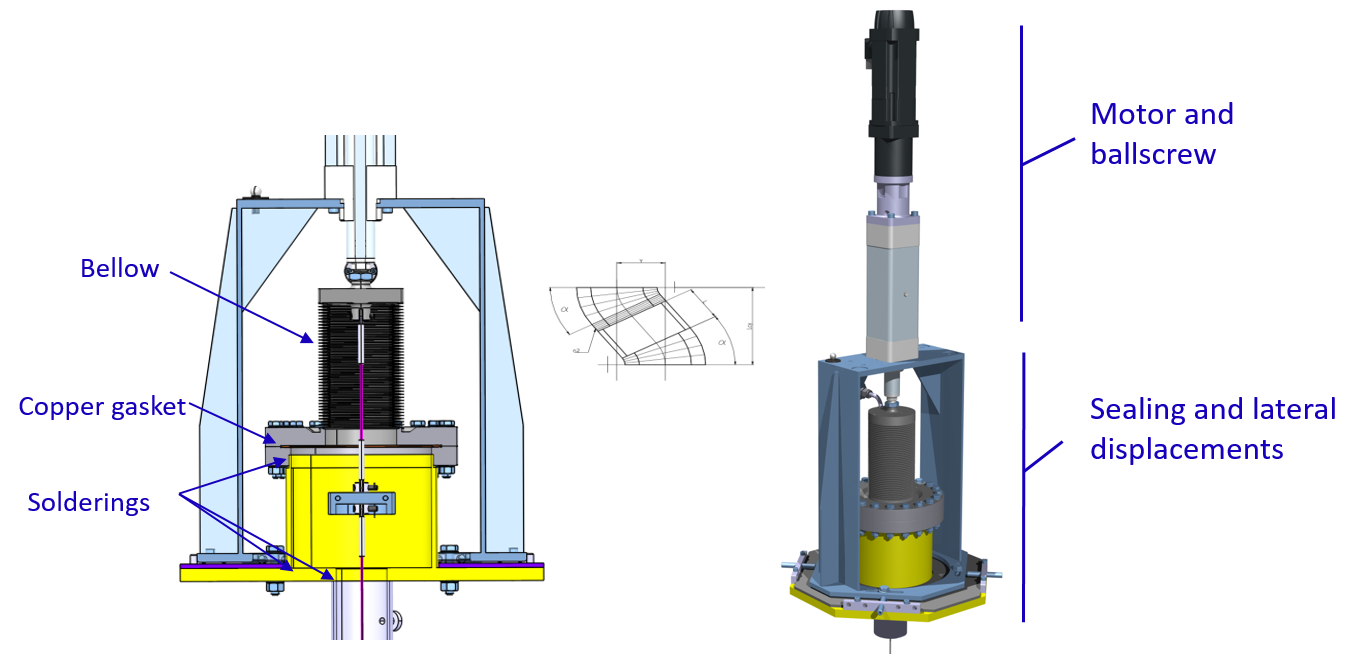
\includegraphics[width=0.80\textwidth]{spft}
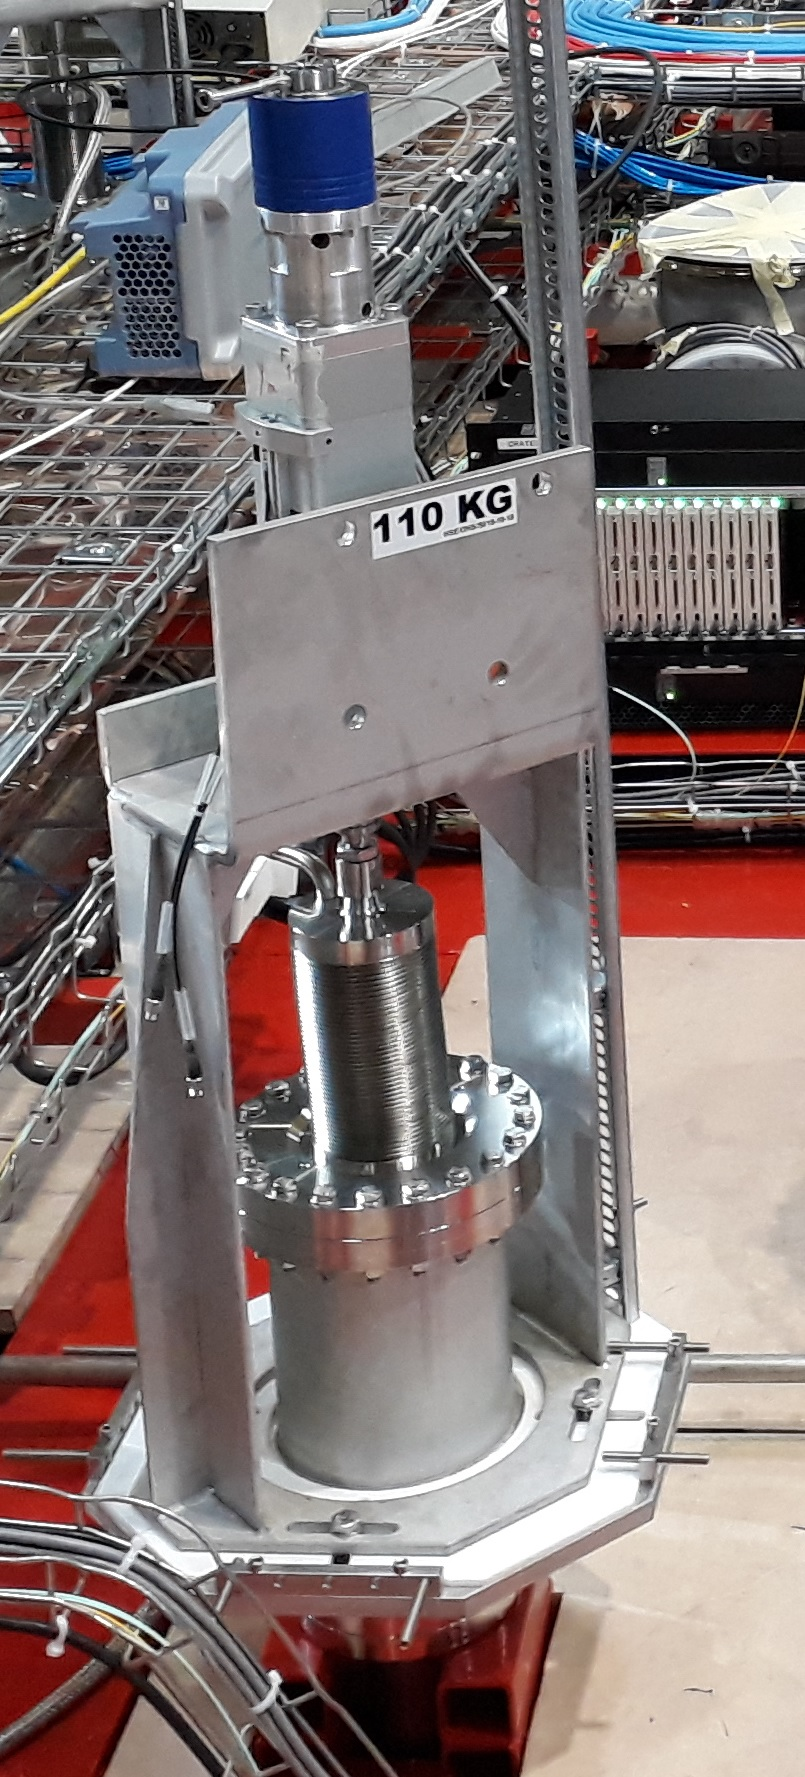
\includegraphics[width=0.19\textwidth]{spft-crp}
\end{dunefigure}
At the level of the flanges on the cryostat roof, the adjusting table to which the suspension \fdth is screwed allows a lateral stroke of \SI{26}{mm}. Any transverse movement is absorbed by lateral deformation of the bellows.
The vertical stroke available with the  size of the bellows is $\pm$\SI{40}{mm}, which corresponds to two times the design specification.
The system incorporates a  mechanical stop and a simple obstruction of the chimney for maintenance or to replace the bellows.
At the top pf the suspension \fdth is a special slot to position a laser tracker target,
so the \fdth position can be precisely surveyed during installation.

Figure~\ref{fig:anchor} shows the suspension cables anchoring system on the \dword{crp} in both a CAD drawing and in a photograph of a \dword{crp}. 
In case of variation in the verticality of the cryostat pipes, this system allows changing an anchoring point on a module in warm conditions. In cold conditions, transverse movement uses the suspension \fdth position adjustment.
\begin{dunefigure}[Anchoring system of the suspension cable on the CRP frame]{fig:anchor}
{Anchoring system of the suspension cable on the \dword{crp} frame.}
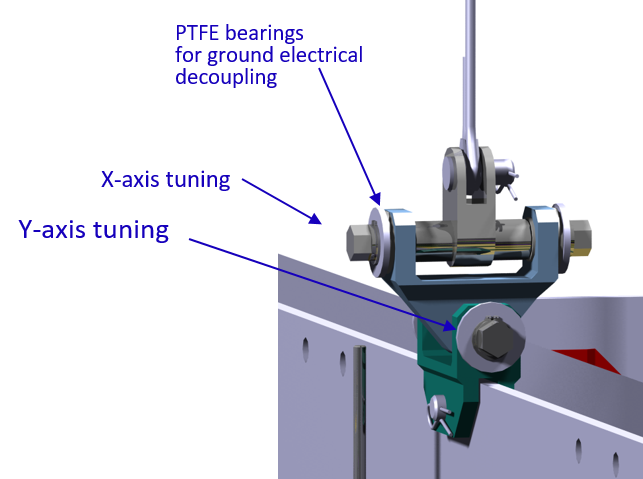
\includegraphics[width=0.55\textwidth]{anchor}
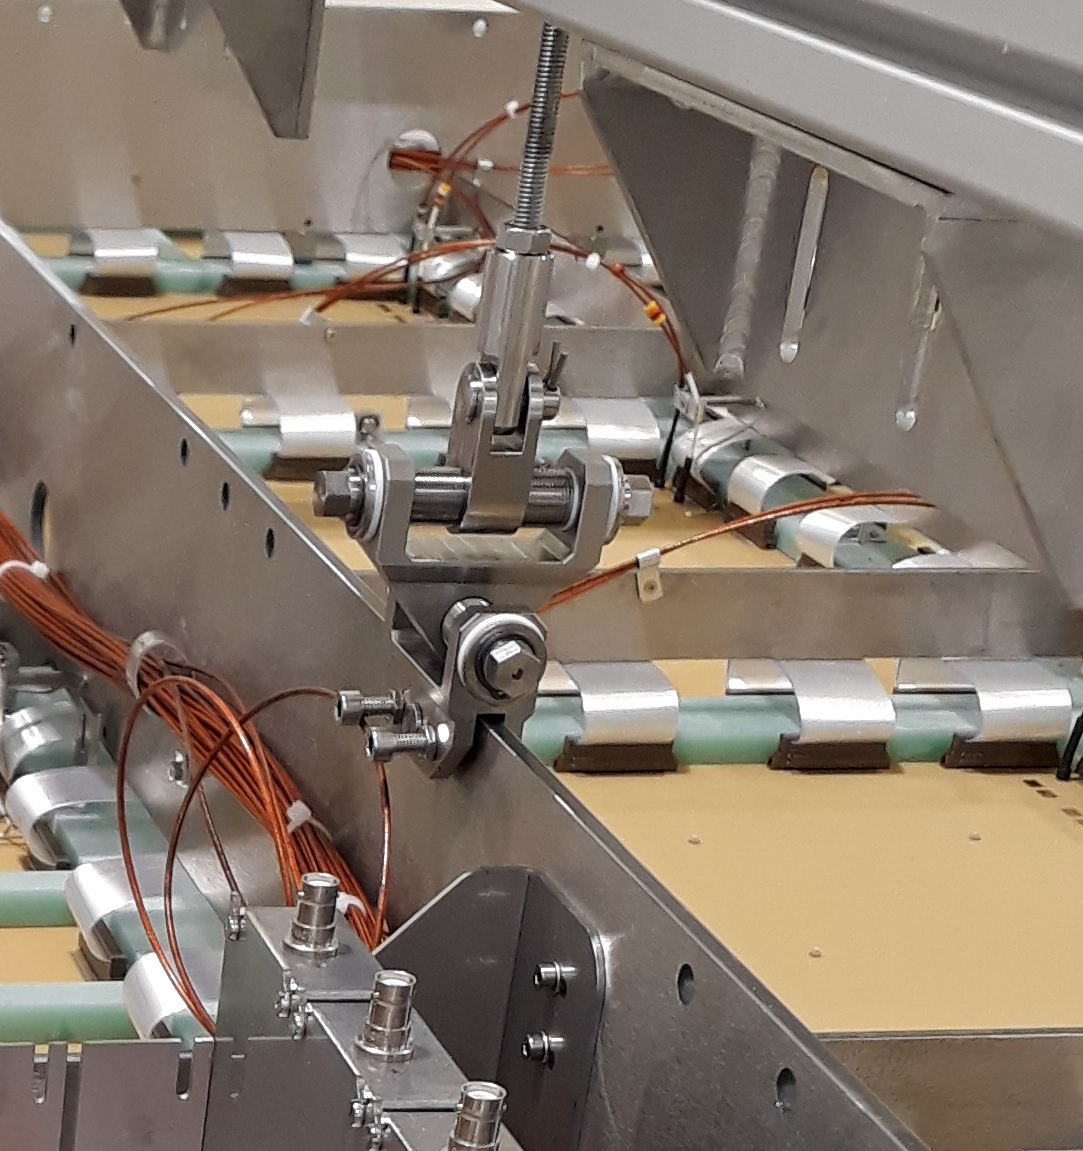
\includegraphics[width=0.44\textwidth]{anchor-crp}
\end{dunefigure}
Each motor has independent controls for tuning the horizontality of the plane using the level information output from the  
sensors. In standard, stable running conditions, several \dword{crp} modules are associated together as a global system and controlled automatically.

%%%%%%%%%%%%%%%%%%%%%%%%%%%%%%%%%%%%%%%%%%%%%%%
\section{Production, Assembly, and Quality Insurance}
\label{sec:dp-crp-prod-assy}

%%%%%%%%%%%%%%%%%%%%%%%%%%%%%%%%%%
\subsection{G10 and Invar Frame Production}
\label{sec:dp-crp-frame}

% new from DD
The G10 and Invar frames are both produced by industry. For the \dword{dpmod}, %80
\dptotcrp Invar frames and \dpnumpmtch %720 
G10 subframes of \SI{1}{m$^2$} are required. 
For \dword{pddp}, the process and \dword{qc} procedures have been defined.
For the Invar structure, SDMS\footnote{SDMS\texttrademark{}, \url{www.sdms.fr/en}.}, the company chosen for \dword{pddp}'s four \dwords{crp},   
has produced them within the specifications without identifiable problems.
They have procured raw Invar plates, which depended on available world stock, planning ahead for the \dword{dpmod}. 
The manufacturing process followed by the manufacturer (SDMS) had eight steps:\\
\begin{itemize}
\item plate rectification,
\item  laser cutting,
\item  assembly,
\item  welding,
\item  geometrical controls,
\item  washing,
\item  packing, and
\item  shipping.
\end{itemize}

During the process, a full-size test frame was built as a special validation step to verify all technical aspects and conformity to requirements. 
Acceptance tests are performed on the geometry, the welding quality, and the proper positioning of the different holes made in the Invar beams.

For \dword{pddp}, fabricating the G10 frames for the four \dwords{crp} was done by a company with expertise in composite materials. The manufacturing process includes  
producing frames made of fiber layers in different orientations as explained in Section~\ref{sec:invar-frame}, drilling more than \num{100} screw threads per square meter of G10 frames, among them \num{80} with a \SI{2}{mm} diameter.
The acceptance tests are mostly based on geometrical and dimension criteria and quality of the threads.  
Producing the G10 frames takes longer and is more difficult than the Invar structure. G10 production would require a minimum of two production sites, while only one company would suffice to produce the Invar frames.


%%%%%%%%%%%%%%%%%%%%%%%%%%%%%%%%%%
\subsection{LEM and Anode Production}
\label{sec:dp-crp-LASprod}


The construction of a  
\dword{dpmod} involves producing \dpnumswch charge readout modules, each made using a \dword{lem} and its anode. For such large production, using more than one manufacturer is desirable to mitigate risks and costs. The ELTOS\footnote{ELTOS\texttrademark{} \url{www.eltos.com}.} company in Italy manufactured the \dword{lem} modules and the anodes for  \dword{pddp} and has successfully worked out the \dword{qa} and \dword{qc} processes based on requirements and specifications of the \dword{wa105} collaboration. The fraction of rejected \dword{lem} modules produced by ELTOS after the final phase of tests was small, fewer than one \dword{lem} per \dword{crp}. The rejection factor for the anodes was, however, higher, approximately \SI{10}{\%}, because of the very thin and fragile conducting strips forming the anode plane as well as the close proximity of the outer strips to the \dword{pcb} edges. 

Small modifications to the anode design for the \dword{dpmod} will be necessary to increase the robustness of the manufacturing process. Such modifications are possible without  
affecting the performance of the anode. These include, for example, the use of larger copper strips on the top face of the anode, allowing for more robust signal connections and of larger inactive edges in order to facilitate the final cutting operation of the PCB.    

A second manufacturer, ELVIA\footnote{ELVIA\texttrademark{} \url{https://www.pcb-elvia.com/}.} in France, can also produce \dwords{lem} and anodes on a large scale with the requested specifications. Recently, ELVIA has indeed produced several \dword{lem} prototypes and extensive tests have 
demonstrated the same \dword{lem} performance as the ELTOS products.
 One key issue for such a very large production, like the one necessary for \dword{dune}, is establishing thorough \dword{qa} and \dword{qc} processes that can be applied to producing all \dwords{lem}. The definition of the \dword{lem} manufacturing requirements and specifications is naturally an important part of the tendering process. As far as the anodes are concerned, several prototypes have already been manufactured by ELVIA with satisfactory results. Despite the size (\num{50}$\times$\SI{50}{cm$^2$}) of the anode, its fabrication follows a rather standard process mastered by several \dword{pcb} manufacturers in Europe and around the world.     

%%%%%%%%%%%%%%%%%%%%%%%%%%%%%%%%%%
\subsubsection{LEM production and QA and QC}
\label{sec:fddp-crp-LEMprod}

An effective production time of \num{40} weeks per year and a total of two years is assumed. This corresponds to an average \dword{lem} production rate of one \dword{crp} or \num{36} \dword{lem} modules per effective week. The main limitation to the manufacturing speed is the \dword{lem} drilling process. While it is likely that ELTOS and ELVIA can each produce \num{18} \dword{lem} modules per week by assigning dedicated drilling machines, it would still be highly advisable, well before the start of the \dword{lem} production phase, to identify additional manufacturers capable of large-scale productions. 

Based on the experience gained with  \dword{pddp}, the  \dword{qa} and \dword{qc} requirements for \dword{lem} manufacturing should include selecting the base material for the \dword{lem} \dword{pcb}, measuring the thickness of the dielectric material and copper layers before and after the process, controlling the size of the \dword{lem} holes, rims, and outer dimensions, and measuring the electrical insulation across the two faces of the \dword{pcb}.  
Table~\ref{tab:LEM_Tolerance} gives, as an example, the requested tolerance values for the various parameters of the \dword{lem} detectors for  \dword{pddp}. In addition, pre-series productions of several \dword{lem} modules from each manufacturing site will be necessary to validate the complete fabrication process before starting full production.

\begin{dunetable}[Tolerance values on various LEM parameters]
{p{.4\textwidth}p{.30\textwidth}}
{tab:LEM_Tolerance}
{Tolerance values on various \dword{lem} parameters.} 
Parameter & Value and tolerance \\ \toprowrule
 
Dielectric thickness & \num{1.00}$^{+0.00}_{-0.05}$\,mm \\ \colhline

Average total thickness & \num{1.20}$^{+0.00}_{-0.06}$\,mm \\ \colhline
 
Dimensions & \num{499.5}$^{+0.00}_{-0.30}$\,mm$\times$499.5$^{+0.00}_{-0.30}$\,mm \\ \colhline

Final PCB thickness & \num{1.10}$^{+0.02}_{-0.05}$\,mm \\ \colhline
 
Active hole diameter & \num{0.50}$^{+0.00}_{-0.01}$\,mm \\ \colhline

Rim size & \num{40}$\pm$4\,$\mu$m \\ \colhline
   
Electrical insulation & >\SI{1}{\giga\ohm} \\
 \end{dunetable}

Once manufactured, the \dword{lem} modules are shipped to one or several collaboration sites for final characterization and validation. The necessary infrastructure includes a survey bench, clean rooms, storage rooms, cleaning stations, and \dword{hv} test set ups. The following is a list of tasks to validate and characterize the modules in sequence:

\begin{itemize}
\item {\bf Visual inspection and survey:} After receiving the \dword{lem} modules from the manufacturer, a visual inspection examines the quality of the \dword{lem} surfaces 
followed by the detector survey. The parameters that determine the \dword{lem} amplification gain are the thickness of the \dword{pcb} and the geometry of the holes. The uniformity of these parameters must be assessed over the entire area of a \dword{lem} module. For  \dword{pddp}, this is done by sampling the modules and assessing with a confocal laser scanning microscope. Several hundred measurements are done in each of \num{25} predefined locations distributed uniformly over the \dword{lem} surface. With such an optical system, the total \dword{lem} and copper layer thicknesses as well as the rim size can be precisely measured within a few microns.  For the magnitude of production required for a \dword{dpmod}, developing a fully automated survey system, similar to what is being used at CEA/Irfu for the New Small Wheel Project of ATLAS, is mandatory. 

\item {\bf \dword{hv} connection:} The next step consists of soldering the \dword{hv} connection pins on the two \dword{lem} copper surfaces as well as gluing the MACOR insulators around the connectors.

\item {\bf Cleaning and polymerization:} Cleaning is an important phase of \dword{lem} preparation. Following a procedure defined by CERN/EP-DT-EF-MP and CEA/Irfu,

 this step uses an ultrasonic bath at $\SI{65}{^\circ{}C}$ with a micro-finishing solution (NGL 17.40 Sp ALU III) to clean the gold-plated copper surfaces of the \dword{lem}. This is followed by rinsing with water and then with a spray of pressurized deionized water 
 ($<$\,30\,bar). The \dword{lem} is then dried in an oven 
at $\SI{60}{^\circ{}C}$  for several hours and then baked for three hours up to $\SI{160}{^\circ{}C}$,  
a temperature near the glass transition point of the dielectric material. From the cleaning operation on, each \dword{lem} is handled using an aluminum frame on which it is mounted to avoid any contact with the \dword{pcb} surfaces. The \dwords{lem} are also 
handled in a clean environment using, for example, a laminar flow.  

\item {\bf \dword{hv} tests:} The final validation of a \dword{lem} requires successful and stable operation in pure argon at room temperature and an absolute pressure of about \numrange{3.2}{3.3}\,bar. A high pressure vessel is used for this.  The argon pressure value is precisely adjusted as a function of the argon temperature inside the vessel to reach the same gas density as the one existing in D\dword{lar} mode. In this way, the \dword{lem} modules are tested at the same Townsend avalanche operation point as in cold. Figure~\ref{fig:HP} shows the \SI{360}{L} high-pressure vessel used at CEA/Irfu to characterize the  \dword{pddp} \dword{lem} modules. Up to nine \dword{lem} modules can be stacked inside this chamber for the \dword{hv} tests. The high-pressure vessel is also instrumented with \dword{fe} electronics and a \dword{daq} system for gain measurements in pure argon. In this configuration, a single \dword{lem} is installed with its \twod charge-collecting anode inside 
a \num{50}$\times$\num{50}$\times$\SI{5}{cm$^3$} 
\dword{tpc} along with a collimated $^{241}$Am open alpha source mounted on 
the cathode. Figure~\ref{fig:HP_ED} shows an event display of a \SI{5.5}{MeV} alpha track observed in pure argon gas at an 
absolute pressure of \num{1}\,bar.
%
The \dword{lem} validation \dword{hv} tests require a two-step procedure. After pumping for 
about \num{60} hours down to a residual pressure of \num{10}$^{-4}$\,mbar, the chamber is filled with dry synthetic air, and 
\dword{hv}  up to \SI{4.5}{kV} is applied across the \dword{lem} to 
burn possible residual dust. Then, the vessel is pumped again, and pure argon (graded \num{5.7})
is introduced at an absolute pressure of approximately \numrange{3.2}{3.3}\,bar. Each \dword{lem} module is tested 
and validated to verify that it can reach the value of \SI{3.5}{kV} across the two faces, consistent with amplification gains higher than \num{100} before charging up, with a discharge rate smaller than 3 per hour. The amount of time needed to perform the \dword{hv}  test is 
typically one week for an entire batch of nine \dword{lem} modules. This last figure can probably be increased to \num{12} with a slightly larger volume vessel. 
\end{itemize}

\begin{dunefigure}
[High-pressure vessel for the characterization of the  ProtoDUNE-DP LEM  modules]
{fig:HP} 
{High-pressure vessel for the characterization of the  \dword{pddp} \dword{lem} modules.}
  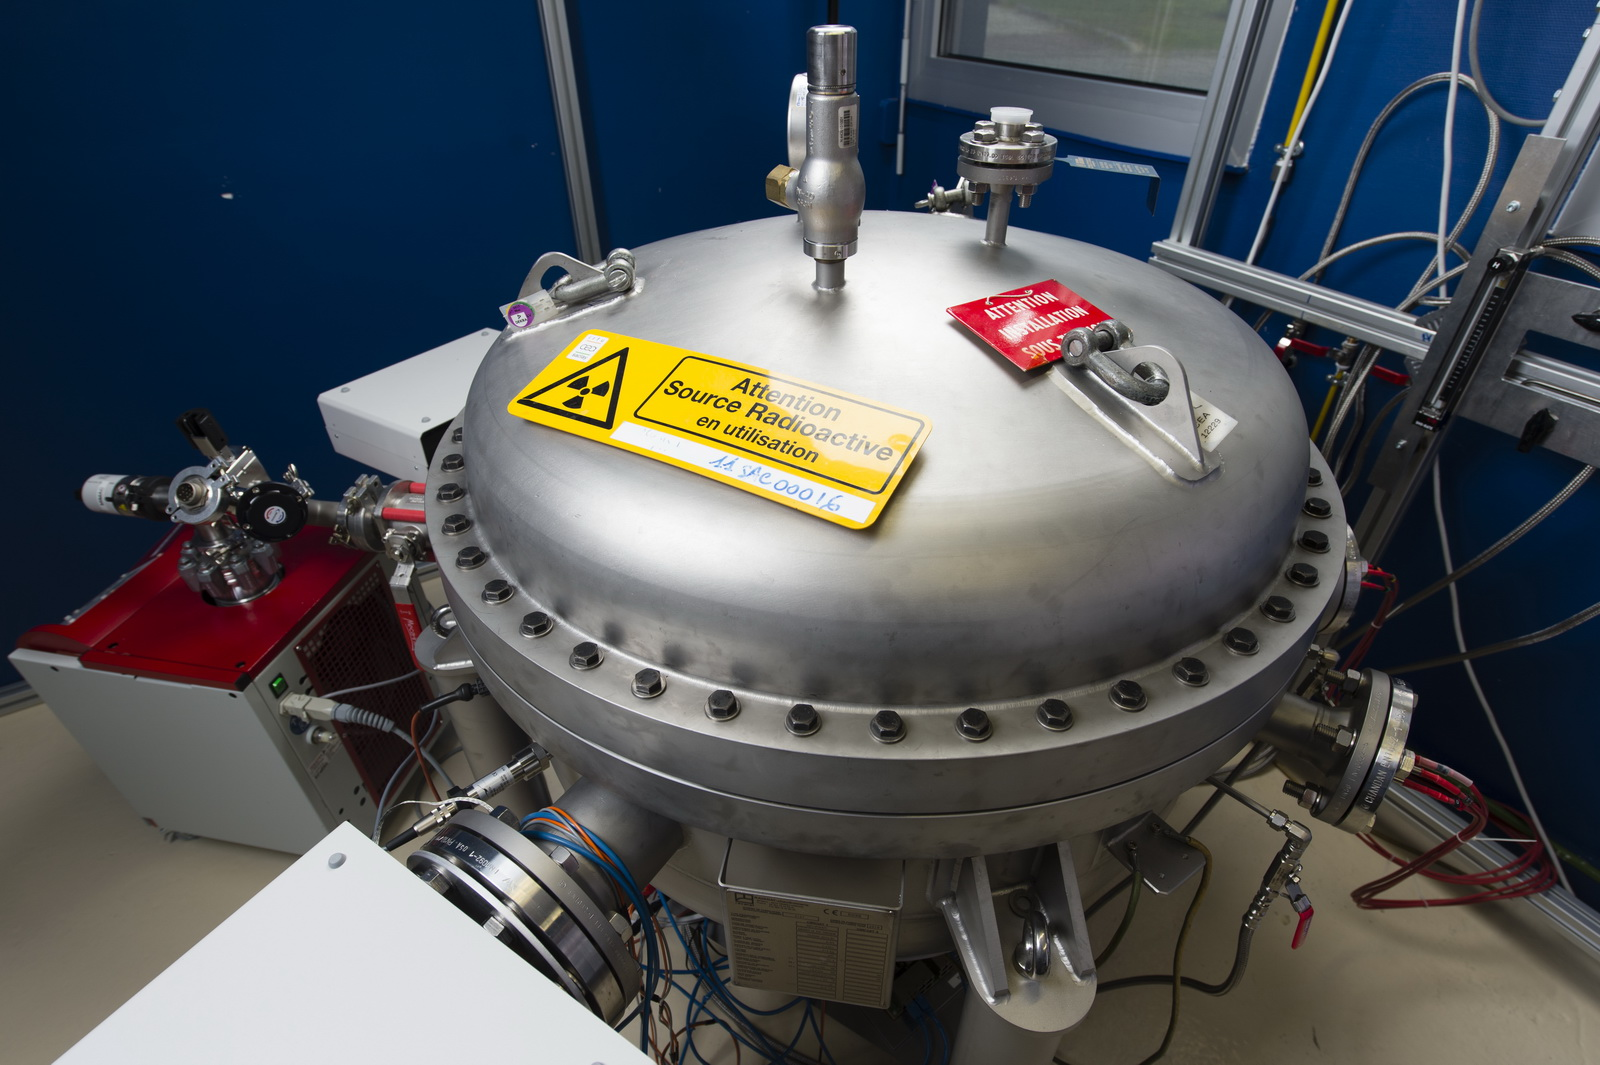
\includegraphics[width=.7\textwidth]{HP}
\end{dunefigure}

While the tasks related to the \dword{lem} visual inspection, survey, and implementation of the \dword{hv} connections can be done at a single participating institution  
, subsequent operations could be divided among several sites. In that case, each 
must have the necessary infrastructure for 
both cleaning and testing because iterations are sometimes necessary to fully validate the 
\dword{lem} modules. Assuming \num{36} \dword{lem} modules produced per effective week, a reasonable number of set ups needed for \dword{hv}  tests, together with associated instrumentation and infrastructure, could be three or four. Finally, based on the experience gained in  \dword{pddp}, the processing time needed to prepare, characterize, and test a batch of nine to twelve \dword{lem} modules is approximately three weeks.  
\begin{dunefigure}
[Event display of a \SI{5.5}{MeV} alpha track in argon gas at \num{1}\,bar.]
{fig:HP_ED}
{Event display of a \SI{5.5}{MeV} alpha track in argon gas at \num{1}\,bar.  Left: $x$-View. Right: $y$-View. Top: Pulse-height distributions of hits in \dword{adc} counts. Bottom: Hit time [300\,ns bins] \textit{vs} strip number.}
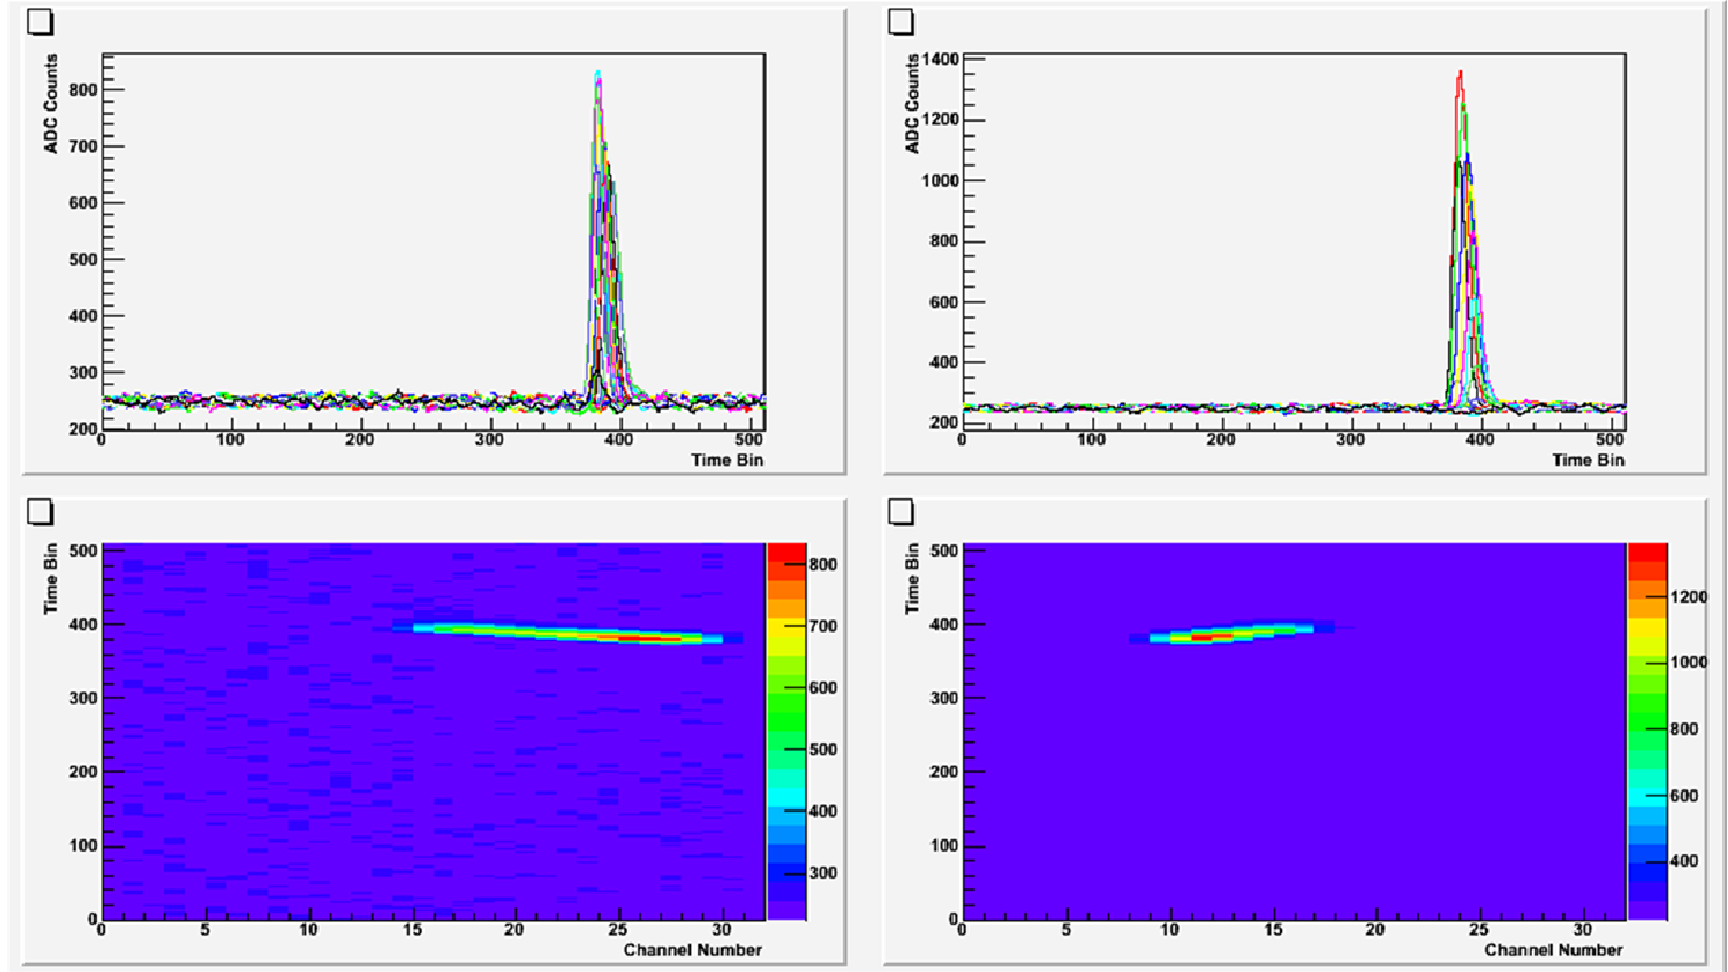
\includegraphics[width=.8\textwidth]{HP_ED}
\end{dunefigure}
%%%%%%%%%%%%%%%%%%%%%%%%%%%%%%%%%%
\subsubsection{Anode production and QA/QC}
\label{sec:dp-crp-ANODEprod}
We can realistically assume that the lead time in manufacturing the anodes will be compatible with the production time
of the \dword{lem} modules. Table~\ref{tab:ANODE_Tolerance} gives the anode specifications for the dimensions of the \dword{pcb}. In addition, we have requested, after the soldering of the signal connectors, visual inspection and continuity tests at the manufacturing site. When the anode strips are received at the collaborating institutions where the \dword{crp} assembly will take place, continuity and short circuit tests of the anode strips are performed (see Figure \ref{fig:Anode_CTest}). This task is rather quick and should not take more than one day per \dword{crp}.  


\begin{dunetable}[Specifications for the anode dimensions]
{p{.4\textwidth}p{.30\textwidth}}
{tab:ANODE_Tolerance}
{Specifications for the anode dimensions.} 
 Parameter & Value and tolerance\\ \toprowrule
 
Dimensions & 499.5$^{+0.2}_{-0.0}$\,mm$\times$499.5$^{+0.2}_{-0.0}$\,mm \\ \colhline

PCB thickness & 3.5$\pm$0.05\,mm \\ \colhline
 
PCB sagitta & < 1\,mm \\
 \end{dunetable}
\begin{dunefigure}
[Test of anode strip continuity]
{fig:Anode_CTest} 
{Test of anode strip continuity.}
 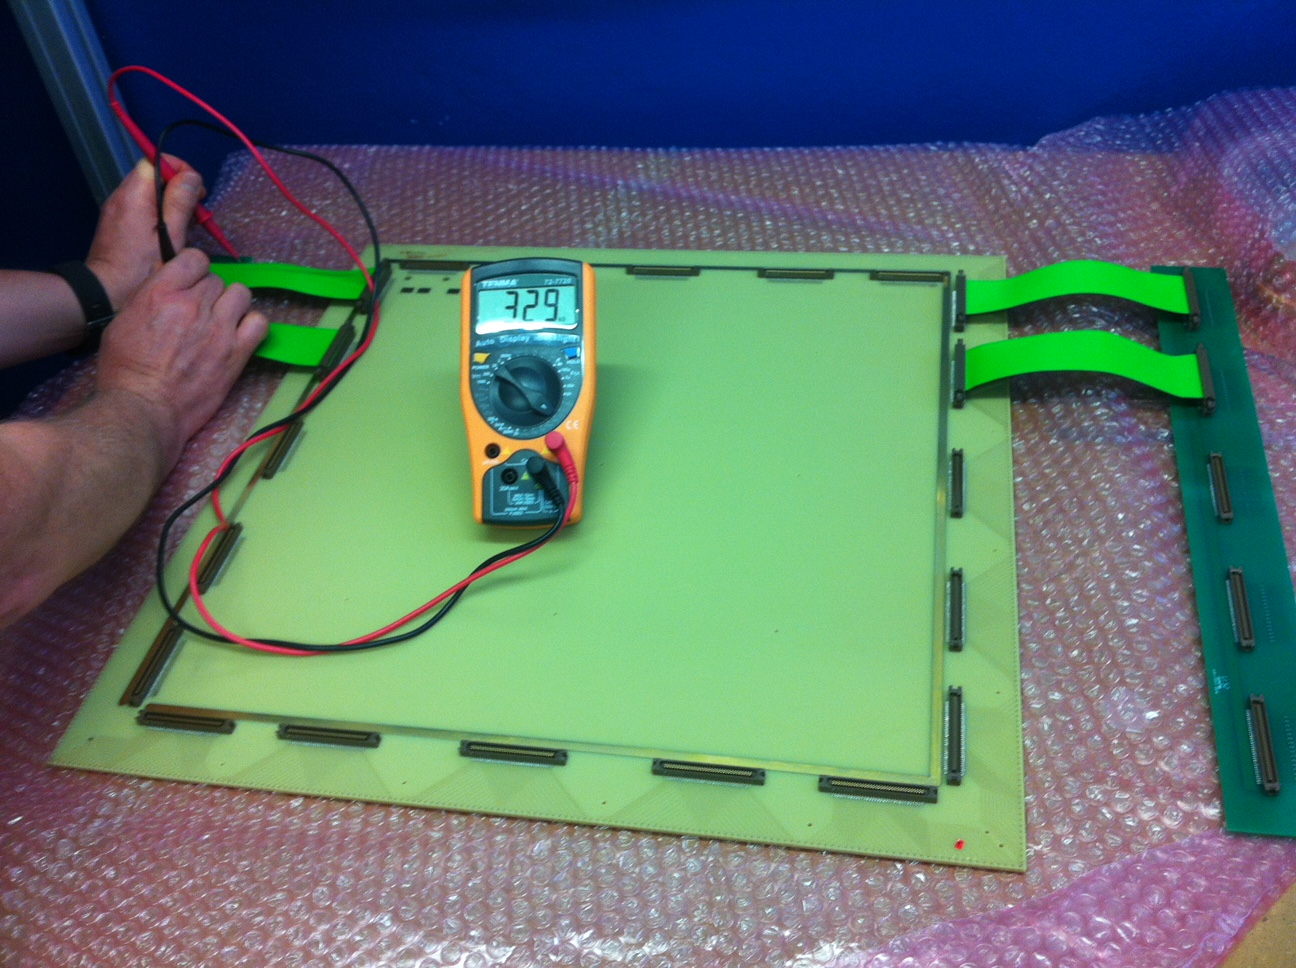
\includegraphics[width=.75\textwidth]{Anode_CTest}
\end{dunefigure}
%%%%%%%%%%%%%%%%%%%%%%%%%%%%%%%%%%
\subsection{Tooling and CRP Assembly}
\label{sec:dp-crp-tooling-assy}
Once the anodes, \dwords{lem}, and the mechanical Invar and G10 frames are produced and delivered, the \dwords{crp} production site should be equipped with several toolings.
The \dwords{crp} construction requires a clean room large enough to accommodate the different work spaces. Separate work areas are required in this clean room for 
\begin{itemize}
\item{A \SI{10}{m$^2$} table for assembling the G10 subframes and for surveying the whole structure;}
\item{A supporting structure from which to hang the Invar frame to couple the G10 frame and install the anodes, \dword{lem}, and extraction grid modules;}
\item{Storage for the anodes and \dwords{lem} on special shelves;}
\item{Space to construct the extraction grid modules and store them before mounting them on the \dword{crp} structure.}
\end{itemize}
The required tooling includes two mobile cranes (\SI{4}{m} span) to manipulate the Invar frame; an aluminum support frame and parts of the transport boxes; a large assembly table; storage shelves for the \dword{lem} and anodes as well as for cables; and a fabrication bench for extracting grid modules.

The \dword{crp} assembly production activity will span two years 
before the \dwords{crp} are installed underground at \dword{surf}. The \dwords{crp} will be integrated in at least two different production sites and stored locally in temporary storage boxes before being shipped to the \dword{surf}. 
The \dword{crp} assembly will be pipelined with the \dword{lem} and anode production and testing during these two production years with an initial  shift of three months. This is intended to constitute a large enough buffer between assembling the \dwords{lem} and anodes before starting \dword{crp} assembly. The baseline scenario should be to assemble two \dwords{crp} in parallel at each assembly site. The tooling and the work space should be adapted to allow it.


Assembling a \dword{crp} in the clean room is a process that begins upon receiving the Invar frame and ends with the  closing of the transport box. 
The \dword{crp} assembly is divided in eight main steps:
\begin{itemize}
    \item  Assembling the G10 frame on the optical table from \num{9} sub-frames  and installing all inserts and coupling screws;
\item Geometry survey of the G10 frame to determine the size along the two directions;
\item Positioning the Invar frame  
above the G10 frame and connecting them through \num{50} decoupling systems;
\item Routing the \dword{lem} \dword{hv} cables;
\item Assembling \dwords{lem} and anodes (done from below), cabling, and \dword{hv} testing;
\item Connecting anodes with jumpers;
 weaving and soldering the extraction grid on the special tooling (done in parallel); then either storing the grids on shelves, or immediately installing them on the \dword{crp};
\item Geometry surveying and tuning of the planarity.
\end{itemize}

The timing needed, the validation at the different steps, and the defining of \dword{qc} and assessments have been done in the context of the \dword{pddp} \dword{crp} construction at \dword{cern} in \num{2018}. The construction  steps of the first \dword{crp} done at \dword{cern} are summarized in Figure~\ref{fig:assembly}.

\begin{dunefigure}
[Summary of assembly steps for the first ProtoDUNE-DP CRP]{fig:assembly}
{Summary of \dword{crp} assembly steps done at \dword{cern} for the first \dword{pddp} \dword{crp}.}
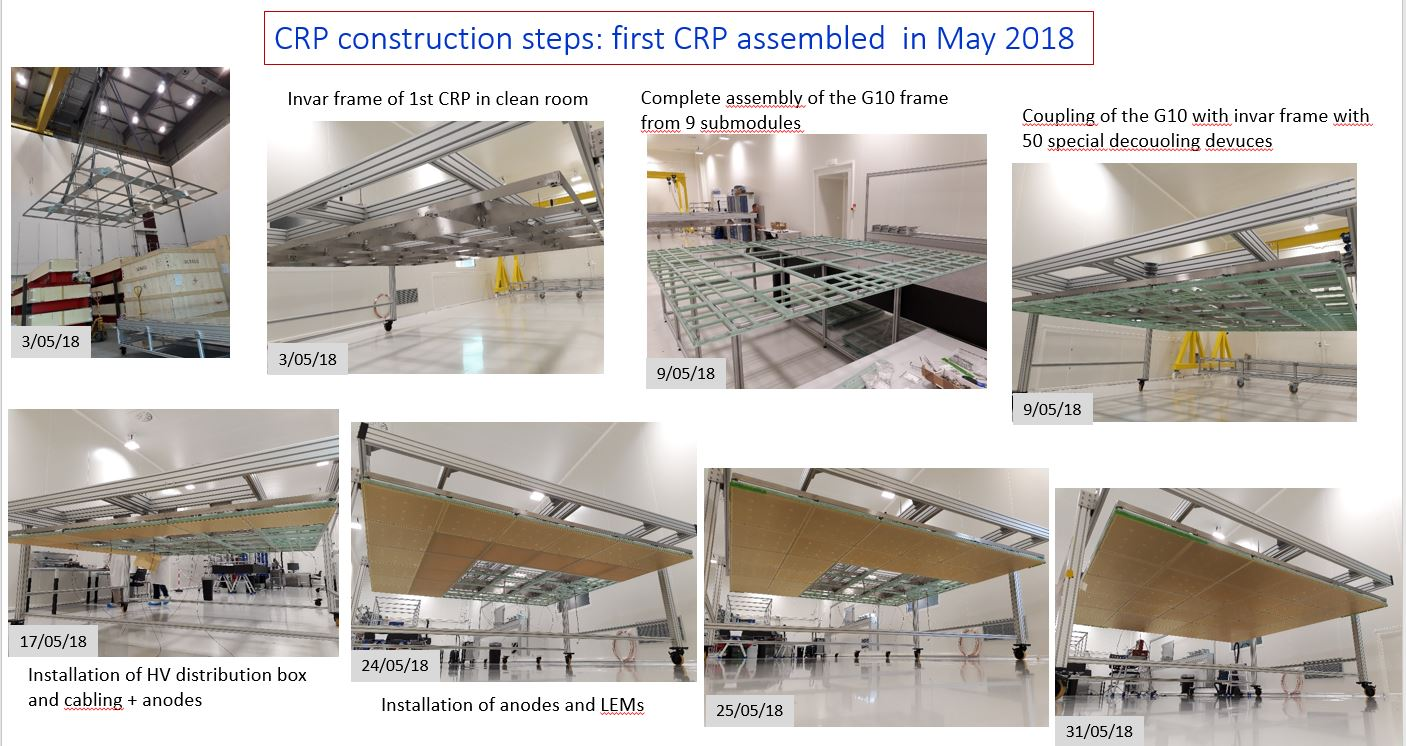
\includegraphics[width=0.98\textwidth]{CRP-steps}
\end{dunefigure}

The \dword{pddp} experience showed us that a \dword{crp}  can be built in four weeks. For the first \dword{crp}, the G10 frame assembly 
took several days to guarantee its flatness and
 to add all the fixation elements before coupling the Invar frame and anodes. In the future, the number of drilled holes and elements to do the assembly can be reduced. This will ease the work and significantly reduce the time needed for this step.
Before the coupling to the Invar structure, the G10 frame underwent a precise metrology to know the size of the frame with a precision  to at least \SI{0.1}{mm}  along both directions. Those measurements are necessary  to adjust the length of the grid weaving tool, so the grid modules have exactly the length required for a 
nominal tension of approximately \num{1.5} N/wire when the modules are screwed onto the G10 frames.
The tension was originally defined on the basis of the material 
properties and calculations. These original 
calculation foresaw that at \dword{lar} temperature, the G10 should contract less than stainless steel,
which should result in a higher tension at cold temperature. According to that calculation,
 based on values of thermal contraction of the different materials measured on samples in 2016, 
the wire contracts over \SI{3}{m} by approximately \SI{9}{mm} while the G10 contracts by approximately \SI{5}{mm}. As a net result, following this model, 
the wire tension at cold should increase from \SI{1.5}{N} to \SI{4}{N/wire} at 87K.

 Grids were produced at a rate of five modules/day, including weaving, wire soldering on the \dword{pcb} plates, and storing. One module corresponds to \num{64} wires. Completing the \num{30} modules needed for one \dword{crp} and the subsequent
 installation takes about \num{10} working days. Figure~\ref{fig:grid-production} shows the fabrication and installation of
 a module on the G10 structure after installing the \dword{lem} and anode. 
\begin{dunefigure}
[Fabrication and installation of the extraction grid]{fig:grid-production}
{Fabrication and installation of one module of the extraction grid.}
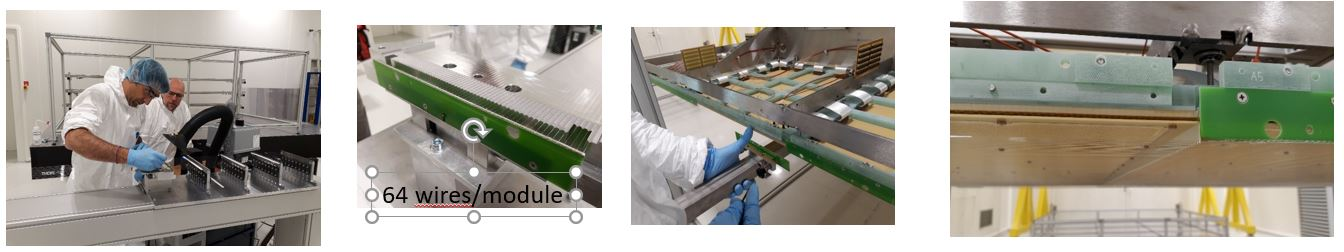
\includegraphics[width=0.98\textwidth]{grid-production}
\end{dunefigure}

Cabling the \dword{lem} \dword{hv}, installing the anode on the G10 frame, and then installing the \num{36} \dwords{lem} 
takes about 5 days. Before the extraction grid is mounted on the G10 frame, anode strip continuity and \dword{lem} 
\dword{hv} connections are tested.

The last operation performed on the \dword{crp} before it is put in its transportation box is the planarity  measurement and adjustment using the \num{50} dedicated screws linking the G10 frame to the Invar frame. The full procedure takes about one day and needs two to three iterations to get a full plane planarity within less than 1 mm. This planarity tuning is repeated in the cryostat before the \dword{crp} is finally raised to its position, thus correcting any possible changes that could have occurred during transportation and manipulation, the \coldbox test, and insertion into the cryostat.
In \dword{pddp}, constructing the four \dwords{crp} benefited from several learning steps and protocol revisions during the first 
assembly, allowing a guarantee of the quality and viability of the whole process for the future.


%%%%%%%%%%%%%%%%%%%%%%%%%%%%%%%%%%%%%%%%%%%
\section{Transport, Handling, and \coldbox Test}
\label{sec:dp-crp-transport}

\subsection{Transport and Handling}
 \label{sec:dp-crp-transport-hand}
 
The transportation boxes are (\num{3.5}$\times$\num{3.5}$\times$\SI{0.8}{m}), so they fit the shafts and can be handled underground at \dword{surf}.
They are protected by a plastic layer that should be removed once the transportation box arrives at the clean area 
underground. The transportation box is essential for manipulating the \dword{crp} from a vertical orientation (i.e., for storage and for insertion into the \dword{tco}) to the horizontal orientation, required 
 before it is hung from the suspension system and for the cold test. Once installation is complete, the transportation boxes are wrapped again with a protective layer and shipped back to the production centers. 

\subsection{\Coldbox Test}
 \label{sec:dp-crp-coldboxtest}
Electrical and mechanical tests of each entire \dword{crp} in realistic cryogenic thermodynamic conditions and in reasonably pure argon vapor will be performed underground  before installing the \dwords{crp} in the cryostat. The tests are done in a  specific \coldbox near the \dword{tco} of the \dword{dpmod}. Four \coldbox{}es will run in parallel to test  all \dwords{crp} at a rate of \num{10} \dwords{crp}/month.
The objectives of this global \dword{crp} test are to
\begin{itemize}
\item Characterize the \dword{hv} operation of each \dword{lem};
\item Characterize the \dword{hv} operation of the extraction grid;
\item Test all \dword{hv} contacts from the \fdth{}s to the \dword{lem} and grid connectors;
\item Measure the flatness of the \dword{crp} before and after cooldown.
\end{itemize}
The \coldbox{}es will be similar to the one developed and built at \dword{cern}  to test the \dword{crp} of \dword{pddp}. Some details can be found in Chapter~\ref{ch:dp-tc}. 

While fabricating and  implementing the initial configuration of the main components, the \dword{protodune} \dwords{crp} underwent very important tests in
the \coldbox. The \coldbox tests allowed correcting and preventing issues with the \dword{crp} design in a continuous improvement process and accumulating significant  experience in the \dword{hv} operation of the \dwords{lem} and extraction grid.
The procedure for the tests begins with opening the transport box to attach the \dword{crp} to the \coldbox roof using the three anchoring points.
 When the cabling and instrumentation of the \dword{crp} is complete,  the \coldbox roof with the the \dword{crp} attached is moved from its garage position to insert the \dword{crp} and close the box as shown in Figure~\ref{fig:dp-crp-coldbox}. 
 
 \begin{dunefigure}
[Insertion of a CRP in the \coldbox]{fig:dp-crp-coldbox}
{Inserting a \dword{pddp} \dword{crp} in the \coldbox at \dword{cern}.}
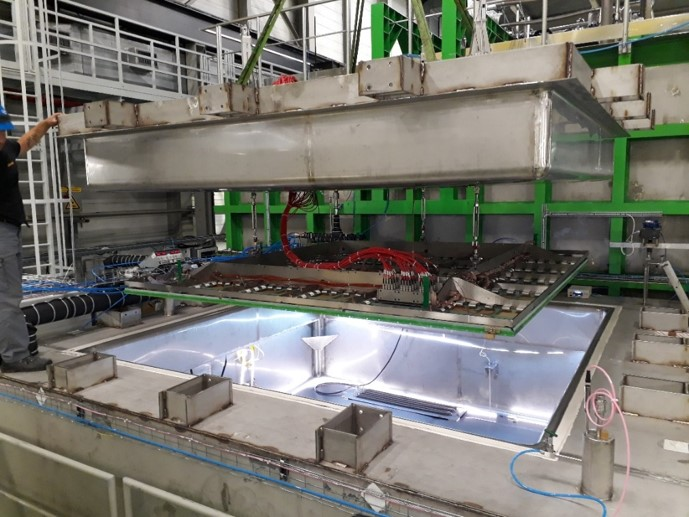
\includegraphics[width=0.8\textwidth]{CRP-coldbox}
\end{dunefigure}

After closure, the \coldbox is filled with dry air to remove humidity and to perform a first \dword{hv} test of the \dwords{lem}. This step burns off possible residual dust on the \dword{lem} surfaces. Typical voltage values above 3000\,V can be achieved across the \dword{lem} electrodes.

Once the \coldbox is filled with \dword{lar} the operational sequence is as follows:
A simplified version of the suspension system allows adjusting the position of the \dword{crp} with respect to the \dword{lar} level using three manual winches to change the height of the \dword{crp} at the level of the anchoring points by steps of \SI{0.4}{mm}.
When the liquid reaches the extraction grid height, the first operation is to adjust the horizontality using temperature probes attached to  the four corners of the grid and information from level meters attached along the four sides of the \dword{crp}. The nominal position is obtained after about one hour, and the cryogenic regulation on the \dword{crp} level meter is then activated. Figure~\ref{fig:dp-crp-incold} shows an image of one \dword{pddp} \dword{crp} tested in the \coldbox after its level was adjusted and the regulation was started. The flatness of the liquid surface is clearly visible and is well below the expected \coldbox requirement.

\begin{dunefigure}
[Camera view of the CRP in the \coldbox]{fig:dp-crp-incold}
{Camera view of the \dword{crp} side where the grid is in the liquid and the \dword{lem} in the gas at the nominal position.}
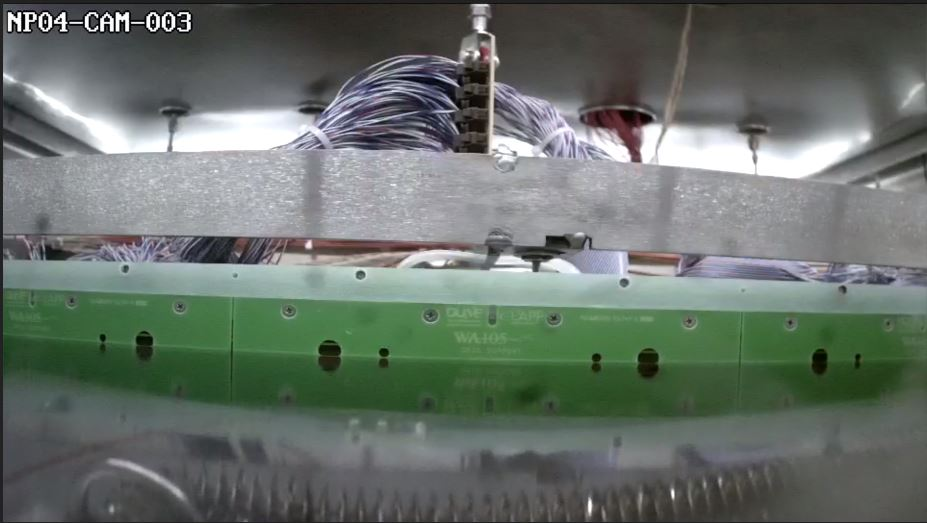
\includegraphics[width=0.7\textwidth]{camera3}
\end{dunefigure}

A  complete \dword{crp} test cycle in the \coldbox typically requires eight days. The \dword{hv} across each \dword{lem} is ramped up slowly until the estimated gain, before charging up of the dielectric, exceeds the nominal value of \num{20}. Because the \coldbox is an open box, the estimated gain depends on the atmospheric pressure, which is constantly monitored. The voltage applied to the extraction grid is about 3000\,V above the value applied to the bottom electrodes of the \dwords{lem}. The \dword{hv} ramping up phase usually takes one or two days. Then, the \dword{crp} is monitored for several days to check its \dword{hv} operation stability; discharges occurring through the \dwords{lem} are recorded. The discharge probability under these \dword{dp} conditions should be less than one per hour for the entire \dword{crp}, corresponding to an average discharge rate of one every \num{36} hours for a single \dword{lem}.

If the test is successful, the \dword{crp} is removed and put in a box to be inserted inside the cryostat. If a problem occurred during the cold test, the \dword{crp} is removed and transported to dedicated area for control and repair. 

%%%%%%%%%%%%%%%%%%%%%%%%%%%%%%%%%%%%%%%%%%%%
\section{Installation, Integration, and Commissioning}
\label{sec:dp-crp-install}
Following the installation of the signal chimneys, which will take three months, installing the \num{80} \dwords{crp} in the cryostat will take eight  months. The signal chimneys must be present in order to 
connect the \dword{crp} signal flat cables. The suspension, instrumentation, and \dword{hv} flanges must also be  installed before the \dword{crp} is installed. These flanges can be installed in parallel with the signal chimneys. 

Production of the \dwords{crp} will start before installation, and the \dwords{crp} will be stored in temporary storage boxes at the production centers. During installation, the already produced \dwords{crp} will be moved to transportation boxes and shipped to \dword{surf}, which is used as a delivery destination buffer, and then  moved underground for testing and installation. Given an installation rate of ten \dwords{crp}/month, a set of \num{40} transportation boxes will ensure sufficient turnover among production sites and the installation site.

The installation procedure  calls for three two-person teams working in parallel inside the cryostat to install three \dwords{crp} at a time. Assuming that 
approximately \num{1.3} weeks is needed for a team to prepare, survey, tune, and cable a \dword{crp} in the  cryostat, all \dptotcrp \dwords{crp} will be installed over \num{32} working weeks.

Once three \dwords{crp} are ready to be lifted, three people must manipulate the manual winches on the top of the cryostat for a few hours. This step occurs during the \num{1.3} week just before  connecting the \dwords{crp} to the flanges. 

The sequence of operations in the cryostat per \dword{crp} is much like the process in the \dword{pddp}: 
\begin{enumerate}
\item A \dword{crp} module in its transport box is brought to the entrance of the cryostat.
\item The box is hung from the side of the insertion rail and guided through the \dword{tco}.
\item  Inside the cryostat, the \dword{crp} is laid horizontally and rolled below the \dwords{sftchimney}.
\item The structure is suspended from temporary cables coming down from the chimney.
\item The transport box is dismounted and removed.
\item The \dword{crp} planarity is measured and tuned based on the metrology survey.
\item The \dword{crp} is raised up with the manual winches, and then the mechanical stop is assembled.
\item The \dword{crp} is lowered on the mechanical stop.
\item The cabling of the \dword{crp} patch panels to \dword{hv}, signal, and slow control \fdth{}s is done.
\item The winch cable is disconnected  and the winch removed.
\item The bellows is compressed using special tooling.
\item The cable from the bellows is connected with a pin.
\item The compression tool is removed and the bellows attached.
\item The motor is inserted and screwed from the top.
\end{enumerate}
 

Assembly is then complete, and the \dword{crp} is operational.
The lateral and vertical alignment of the \dword{crp} is performed from the top of the cryostat with an SPFT translation mechanism, distance meter measurements, and metrology.

The cabling is done while working at the nominal height position using elevating platforms. Access between two adjacent \dwords{crp} requires staggering the altitude of the two modules by about \SI{20}{cm} allowing enough space to do the electrical connections. 

%%%%%%%%%%%%%%%%%%%%%%%%%%%%%%%%%%%%%%%%%
\section{Interfaces}
\label{sec:dp-crp-interfaces}

The main \dword{crp} interfaces are with the elements connected directly to them. The documents that describe the interfaces are referenced:
\begin{itemize}
\item The readout electronics for the cabling of the signal cables on the bottom part of the cold 
flange of the signal chimneys; 
\item The \dword{cisc} for the power supplies for the \dword{lem} and extraction grid, the cameras, \dword{led} ribbons, temperature sensors, and distance meters; all these devices go to the \dword{crp} instrumentation \fdth{}s; 

\item Drift \dword{hv}, at the level of design requirements, includes the system for maintaining the proper distance between the top-most field shaping profile to the extraction grid to maintain the proper extraction field and protect the contact between the two systems. Another interface is the \dword{hv} \fdth{} and extender assembly that must pass through the \dword{crp} plane to reach the cathode at the bottom of the \dword{crp}.  A pass-through hole in a special corner of the \dword{crp} module is the agreed upon solution.
\end{itemize}

%%%%%%%%%%%%%%%%%%%%%%%%%%%%%%%%%%%
\subsection{TPC Electronics}
\label{sec:dp-crp-intfc-elec}

The interface with the \dword{dp} \dword{tpc} electronics is on the level of the bottom flanges of the \dwords{sftchimney} where the flat cables bringing the signals from the anodes are plugged in while installing the \dword{crp} in the cryostat. The system for 
pulsing the anode strips is installed by the \dword{crp} consortium 
concurrent with installing the \dword{crp}. 
The strips are then calibrated jointly by the two consortia.

%%%%%%%%%%%%%%%%%%%%%%%%%%%%%%%%%%%
\subsection{Instrumentation and HV Feedthrough Flanges}
\label{sec:dp-crp-intfc-FT}

The \num{36} \dword{lem} modules of a \dword{crp} are supplied with \dword{hv} by \num{42} coaxial cables 
connecting the \fdth flange from the top of the cryostat to distribution boxes located on the \dword{crp}. Each cable (\num{20}\,AWG, \SI{50}{\ohm} Kapton\footnote{DuPont\texttrademark{} Kapton, polymide film,  E. I. du Pont de Nemours and Company,  \url{http://www.dupont.com/}.} insulated coaxial cable from ACCU-GLASS\footnote{ACCU-GLASS\texttrademark{}, \url{http://www.accu-glass.com/}.}) can sustain \SI{30}{kV} in air and has \dword{shv} plugs on each end to facilitate connections during \dword{crp} installation.

Six coaxial cables are used for the top \dword{lem} electrodes and \num{36} cables for the bottom ones. Each of the cables for the top \dword{lem} electrodes is connected to a single distribution box, located on the \dword{crp}, that contains a \dword{pcb} for distributing \dword{hv} individually to the six \dword{lem} modules through a \SI{500}{\mega\ohm}, limiting current resistor in series. The \num{36} coaxial cables for the bottom \dword{lem} electrodes are connected individually to the \dwords{lem} through \SI{500}{\mega\ohm} resistors located outside the cryostat, in a distribution box or patch panel that allows the connection of one or more LEM cables to a single channel of the HV power supply. In ProtoDUNE-DP, the choice was made to connect each \dword{lem} bottom electrode to a single power supply channel for flexibility purposes. For the \dword{dp}
module, each HV power supply channel will be distributed to six bottom electrodes in order to reduce the number of channels and cost. Remotely controlled HV power supplies with adequate performance and sensitivity are commercially available.
For ProtoDUNE-DP, the 16-channel CAEN 8kV A1580H modules are 
used for the \dwords{lem} power supplies while a 6-channel CAEN 12kV A1524 module is used to power the extraction grids.  

\begin{comment}
\begin{dunefigure}
[Distribution boxes for the top \dshort{lem} HV]{fig:crp_db2}
{Distribution boxes for the top \dword{lem} HV.}
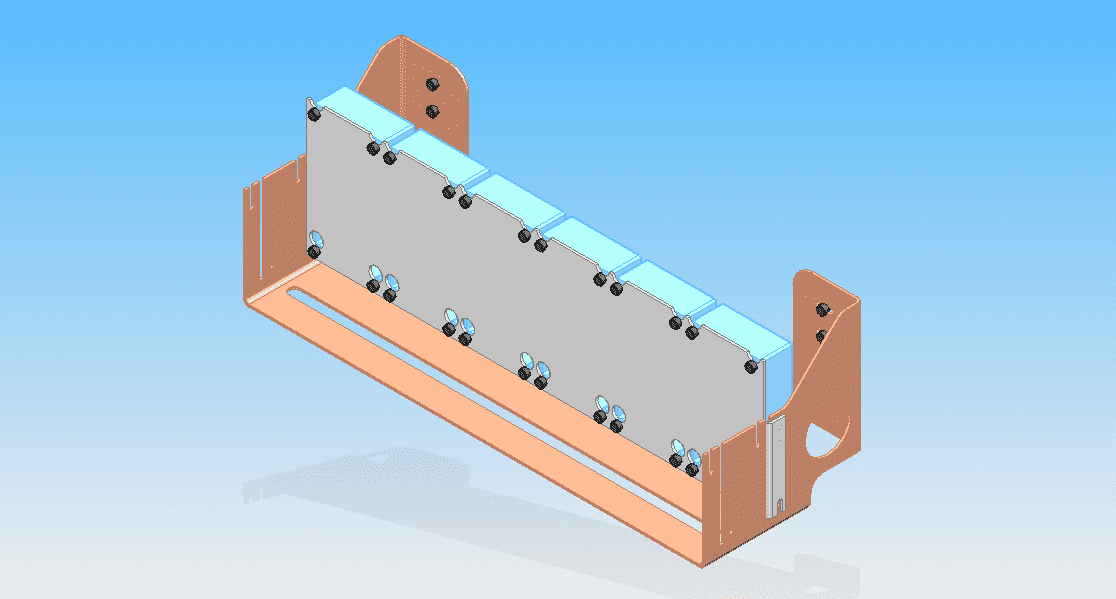
\includegraphics[width=0.6\textwidth]{graphics/CRP_DB2.png}
\end{dunefigure}
\fixme{figure \ref{fig:crp_db2} is not referenced in the text.}
\end{comment}
%%%%%%%%%%%%%%%%%%%%%%%%%%%%%%%%%%% 
\subsection{Cryostat and Detector Support Structure}
\label{sec:dp-crp-intfc-support}

The cryostat includes dedicated penetrations for the hanging system of each \dword{crp}. Each penetration is \SI{100}{mm} in diameter. The layout of the cryostat penetrations matches the position of the hanging points on the \dword{crp} supporting structure. The penetration flanges and \dword{crp} suspension stepper motors are provided by the \dword{crp} consortium.

%%%%%%%%%%%%%%%%%%%%%%%%%%%%%%%%%%%%%%%%%%%%%%%
\section{LEM Improvement Plan}
\label{sec:dp-lem-ip}

CEA/Irfu is collaborating with the EP-DT-DD Micro-Pattern Technologies (MPT) service at \dword{cern} to develop a 
new \dword{lem} design for the second phase of \dword{pddp} and for \dword{dune}. The main goal is to improve the operation reliability and stability of the \dword{lem} detectors following a threefold plan:
\begin{itemize}
\item Improving the micro-etching process to produce better quality rims around the amplification holes;  
\item Increasing the \dword{lem} active area;
\item Reducing the probability of discharges occurring through the amplification holes.
\end{itemize}

The \dword{crp} tests performed in the \coldbox for \dword{pddp} in 2018 revealed some defects in the \dword{lem} rim 
manufacturing, resulting in the carbonization of amplification holes on a few \dwords{lem} during operation. These defects, which affected the operation performance of the \dword{crp}, were found in the corners and the edges of the faulty \dwords{lem}. They are attributed to the micro-etching process used by the manufacturer to produce the rims around the amplification holes. Indeed, in regions of a \dword{lem} where the hole density is not uniform and larger amounts of passive material are present, using chemical baths alone, as it is standard among \dword{pcb} manufacturers, cannot guarantee a uniform rim quality in the periphery of the \dword{lem}. Furthermore, copper residues are often found on the rim edges, causing multiple discharges from the \dword{lem} during operation. Figure~\ref{fig:bad_lems_rims} shows a picture of a \dword{lem} that suffered from carbonization during \coldbox tests. 
\begin{dunefigure}
[\dshort{lem} that underwent carbonization in the \coldbox]{fig:bad_lems_rims}
{Example of a \dword{lem} that underwent carbonization during its operation in the \coldbox (left) and microscopic view of the rims near the edge and corner regions (right).}
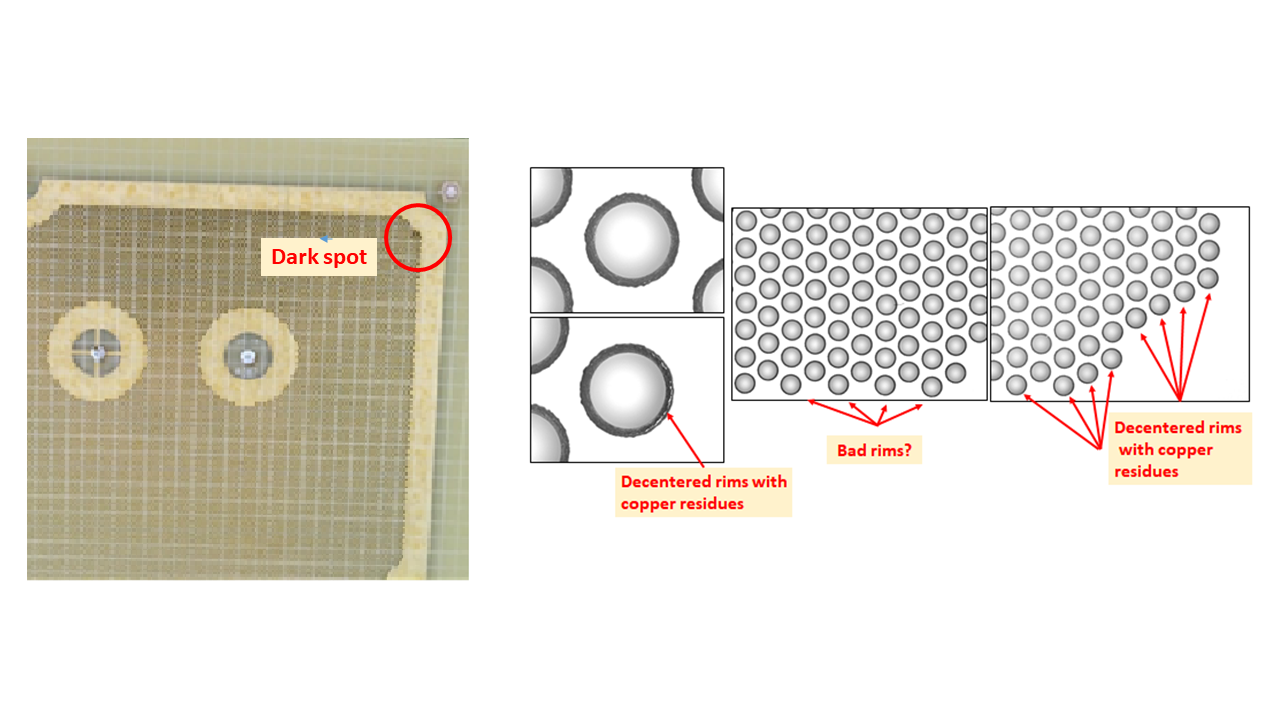
\includegraphics[width=1.0\textwidth]{graphics/BadRIMs1.png}
\end{dunefigure}
    
A new micro-etching process, recently developed by the MPT service at \dword{cern}, avoids these manufacturing issues. Figure~\ref{fig:new_rim_process} shows schematically the various steps of this technique used to 
manufacture the \dword{lem} rims. Figure~\ref{fig:scan_rims} shows a microscopic view of a full scale \dword{lem} made by \dword{cern} with this micro-etching process. As can be seen, high-quality rims could be obtained in the corner regions of the \dwords{lem} with no visible copper residues at the edge of the rims.
Four \dword{lem} prototypes have recently been made by \dword{cern} using this new technique and are now being tested at CEA/Irfu in pure argon gas in the high pressure chamber.

\begin{dunefigure}
[New rim process]{fig:new_rim_process}
{New technique for \dword{lem} micro etching developed at \dword{cern}. (a) Before the drilling phase, the \dword{pcb} is covered by a thin  15\,$\mu$m layer of adhesive copper. (b) A chemical spray is then used to remove the copper layer, leaving a thin, transparent protective glue layer on top of the \dword{pcb} copper. A small rim of the 10-15\,$\mu$m size is initially formed as the chemical spray enters through the amplification holes. (c) The micro etching process is continued until the final rim size is achieved. Control of rim quality and size is possible using the transparent glue film. (d) At the end of the process, the protective glue layer is removed.}
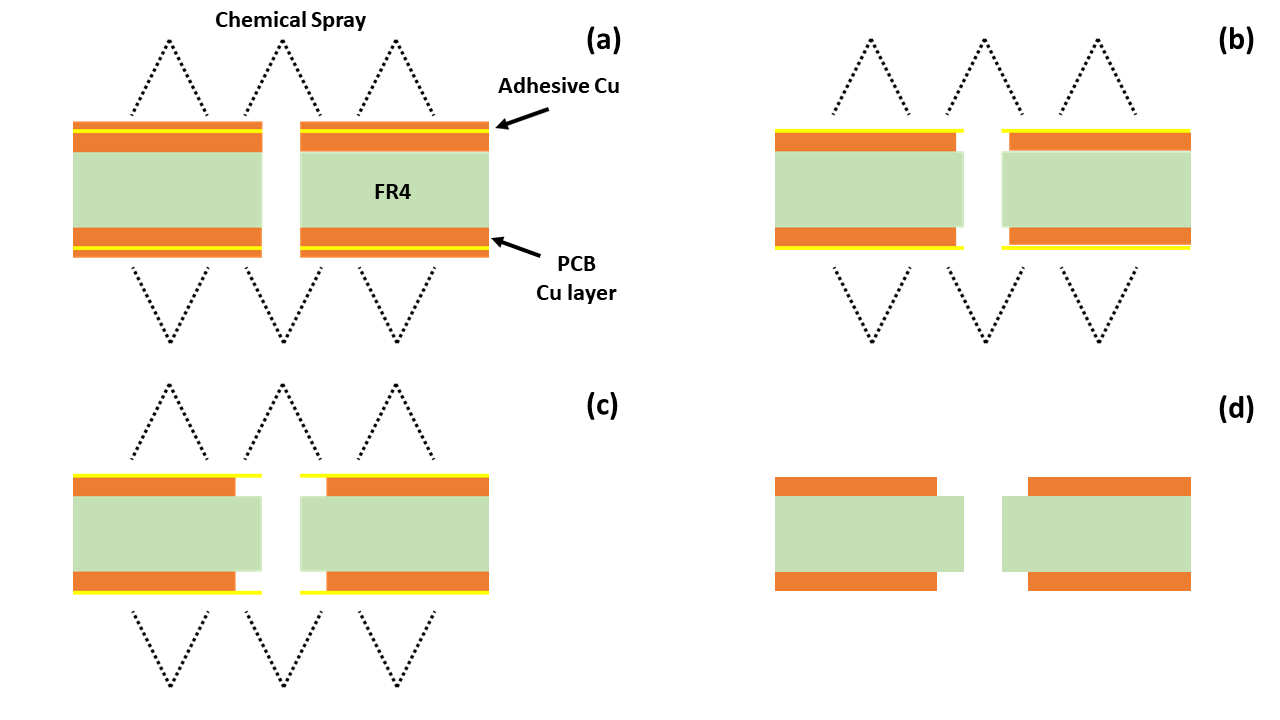
\includegraphics[width=1.0\textwidth]{graphics/NewRims.png}
\end{dunefigure}
\begin{dunefigure}
[New \rms]{fig:scan_rims}
{Microscopic image of a \dword{lem} manufactured with a new micro-etching technique developed at \dword{cern}}.
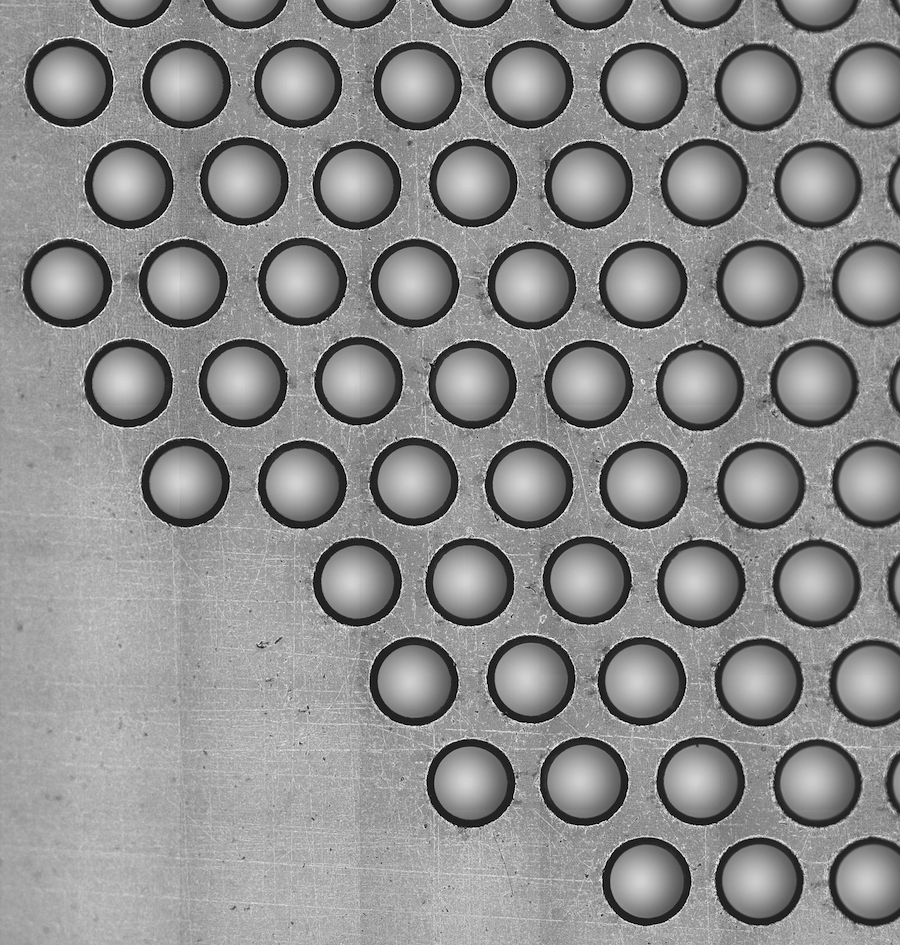
\includegraphics[width=0.5
\textwidth]{graphics/Scan_8.png}
\end{dunefigure}

The \dword{lem} design adopted for \dword{pddp} has an active area limited to approximately 86$\%$. This choice was made to reduce the discharge rate of a \dword{lem}, in particular near boundary regions where the electric field intensity is known to be large. To overcome this and to achieve, in the future, active areas larger than 95$\%$, we propose using an insulation layer covering the regions with no amplification holes. Electrostatic calculations show that such a layer with a few tens of microns thick would be sufficient to significantly lower the field intensity in those regions. In this way, reducing the \frfour clearance and copper guard ring in the peripheral region of a \dword{lem} is possible, as is obtaining a larger active area. Tests with a 65\,$\mu$m adhesive kapton as an insulation material are being carried out at CEA/Irfu. For the final \dword{lem} design, materials compatible with \dword{lar} temperatures, like a solder mask or a coverlay, could be used. Other possibilities are also being considered. These include a modification of the size and the geometry of the amplification holes in the peripheral regions to reduce the electric field intensity near the \dword{lem} borders.

Although \dword{lem} discharge rates lower than one every \num{36} hours have been obtained at effective gains above \num{20} in dedicated \coldbox tests, it is desirable to reduce as much as possible such processes in order to mitigate aging effects. We thus propose testing a new micropattern gaseous detector technology based on the resistive diamond like carbon (DLC) coating. Resistive anode technology has been developed for the International Linear Collider (ILC) \dword{tpc} and is now considered with Micromegas detectors for the \dword{t2k} \dword{nd} upgrade. The resistive MPGD readout technology is well known to be resistant to sparks. Manufacturing a \dword{lem} incorporating resistive technology consists of replacing the copper layer on the bottom face by a kapton foil (typically 50$\mu$m thick) on which a very thin layer (< 1$\mu$m) of DLC is deposited. Such a \dword{lem} prototype is now being constructed at \dword{cern} and will be tested at CEA/Irfu in fall 2019. 

The goal of the \dword{lem} improvement plan is to finalize the \dword{lem} design and to start the manufacturing phase in 2020 to allow a full \dword{crp} test in the \coldbox early 2021 at \dword{cern}.

%%%%%%%%%%%%%%%%%%%%%%%%%%%%%%%%%%%%%%%%%%%
\section{Safety}
\label{sec:dp-crp-safety}

Safety must be a central feature of all tasks performed by the \dword{crp} consortium.  All aspects of \dword{crp} construction, installation, and commissioning will adhere to procedures established by the \dword{dune} \dword{tcoord} and relevant host institutions. 

The \dword{crp} installation and operation does not present particular safety issues apart from working at heights  
while connecting the  \dword{crp} cabling to the \dwords{sftchimney} and instrumentation to the \dword{hv} \fdth{}s.
%%%%%%%%%%%%%%%%%%%%%%%%%%%%%%%%%%%%%%%%%%%%%
\section{Risks}
\label{sec:dp-crp-risks}
The design  of the \dword{crp} takes into account several risks, summarized in Table~\ref{tab:risks:DP-FD-CRP}.
The risk items presented in the table for the \dword{dune} \dword{dpmod} are derived from those that have been  addressed in \dword{pddp}. They have been identified for the production of the \dword{crp} elements, for the assembly, the cold tests, and installation in the cryostat.


 
% risk table values for subsystem DP-FD-CRP
\begin{footnotesize}
%\begin{longtable}{p{0.18\textwidth}p{0.20\textwidth}p{0.32\textwidth}p{0.02\textwidth}p{0.02\textwidth}p{0.02\textwidth}}
\begin{longtable}{x{0.18\textwidth}x{0.20\textwidth}x{0.32\textwidth}x{0.02\textwidth}x{0.02\textwidth}x{0.02\textwidth}} 
\caption[Risks for DP-FD-CRP]{Risks for DP-FD-CRP (P=probability, C=cost, S=schedule) More information at \dword{riskprob}. \fixmehl{ref \texttt{tab:risks:DP-FD-CRP}}} \\
\rowcolor{dunesky}
ID & Risk & Mitigation & P & C & S  \\  \colhline
RT-DP-CRP-01 & Poor quality of G10  frames and/or inaccuracy in the hole machining & Clearly specified requirements, followup and seek out backup vendors & L & L  & M \\  \colhline
RT-DP-CRP-02 & LEM production takes longer than expected & Define a production schedule allowing enough contingencies to limit the assembly impact   & L & L  & M \\  \colhline
RT-DP-CRP-03 & One of the CRP assembly site not ready on time & Close oversight on construction of tooling and preparation of assembly sites & L & M & H  \\  \colhline
RT-DP-CRP-04 & Materials shortage at production site & Develop and execute a supply chain management & M & L  & L \\  \colhline
RT-DP-CRP-05 & Failure of extraction grid winding machine & Regular maintenance and availability of spare parts & L & L  & L \\  \colhline
RT-DP-CRP-06 & CRP assembly takes longer time than planned & Estimates based on ProtoDUNE-DP. Formal training of every tech/operator at each site. & L & M & M \\  \colhline

\label{tab:risks:DP-FD-CRP}
\end{longtable}
\end{footnotesize}
 
%%%%%%%%%%%%%%%%%%%%%%%%%%%%%%%%%%%%%%%%%%%%%%%
\section{Organization and Management}
\label{ch:dp-crp-manage}

\subsection{Consortium Organization}
\label{ch:dp-crp-organization}
The \dword{crp} consortium currently includes three participating institutions that helped in designing, constructing, and assembling the \dword{crp} for \dword{pddp}. The institutions are listed in Table~\ref{tab:dp-crp-institutes}.

\begin{dunetable}
[Participating institutions]
{ll}
{tab:dp-crp-institutes}
{Institutions participating in the \dword{crp}  consortium.}
Institution & Country  \\ \toprowrule
CERN & Switzerland \\ \colhline
CEA/Irfu & France \\ \colhline
LAPP & France \\ 
\end{dunetable}

 The consortium management team consists of one leader (France).

\subsection{Planning Assumptions}
\label{ch:dp-crp-planning}
The present design of the \dword{crp} relies on elements already developed for \dword{pddp} including production, assembly, and installation. 
Commissioning \dword{pddp} in \num{2019} should provide some additional information but should not modify the design philosophy of the main structure and components.  Some changes in the \dword{lem} design, not affecting the general structure, will improve \dword{hv} stability over time as well as increase the active area.  Upgrades of the mechanical structure frames will also simplify the assembly of the G10 part and reinforce the stiffness of the Invar supporting structure. Those changes are being worked out to provide two equipped \dwords{crp} to replace the dummy ones for \dword{pddp} phase II.
Another modification is foreseen for the transport boxes. They are being redesigned to reduce the time needed to insert and extract a \dword{crp} and to allow safe storage in a vertical position.

\subsection{High Level Schedule}
\label{ch:dp-crp-costschedrisk}

The key \dword{crp} schedule milestones are listed in Table~\ref{tab:CRPsched}. The dates given assume the \dword{dpmod} will be the second \dword{fd} module to be installed.
\begin{dunetable}
[CRP  schedule and milestones]
{p{0.65\textwidth}p{0.25\textwidth}}
{tab:CRPsched}
{\dword{crp} consortium schedule.}   
Milestone & Date (Month YYYY)   \\ \toprowrule
\colhline
Test of new CRP with upgraded mechanics and LEMS  in cold box  &   January 2021   \\ \colhline
\rowcolor{dunepeach} Start of \dword{pdsp}-II installation& \startpduneiispinstall      \\ \colhline
Construction of second CRP for ProtoDUNE-DP II & June 2021
 \\ \colhline
\rowcolor{dunepeach} Start of \dword{pddp}-II installation& \startpduneiidpinstall      \\ \colhline
\rowcolor{dunepeach}South Dakota Logistics Warehouse available& \sdlwavailable      \\ \colhline
\dword{prr} dates &   June 2022   \\ \colhline
\rowcolor{dunepeach}Beneficial occupancy of cavern 1 and \dword{cuc}& \cucbenocc      \\ \colhline
Start of tooling production  &   October 2022   \\ \colhline
Start of  Invar and G10 frame production  &    January 2023   \\ \colhline
Start of LEM and anode production  &   January 2023   \\ \colhline
\rowcolor{dunepeach} \dword{cuc} counting room accessible& \accesscuccountrm      \\ \colhline
\dword{crp} assembly sites qualified &   December 2023   \\ \colhline   
\rowcolor{dunepeach}Top of \dword{detmodule} \#1 cryostat accessible& \accesstopfirstcryo      \\ \colhline
Start of  \dword{crp} assembly  &   January 2024   \\ \colhline  
\rowcolor{dunepeach}Start of \dword{detmodule} \#1 TPC installation& \startfirsttpcinstall      \\ \colhline
\rowcolor{dunepeach}Top of \dword{detmodule} \#2 accessible& \accesstopsecondcryo      \\ \colhline
\rowcolor{dunepeach}End of \dword{detmodule} \#1 TPC installation& \firsttpcinstallend      \\ \colhline
 \rowcolor{dunepeach}Start of \dword{detmodule} \#2 TPC installation& \startsecondtpcinstall      \\ \colhline
 Start of  \dword{crp} installation  &   September 2025   \\ \colhline
 End of  Invar and G10 frame production  &    November 2025   \\ \colhline
 End of LEM and anode production  &   November 2025   \\ \colhline
 End of  \dword{crp} assembly  &   January 2026   \\ \colhline
 End of  \dword{crp} installation  &   April 2026   \\ \colhline
\rowcolor{dunepeach}End of \dword{detmodule} \#2 TPC installation& \secondtpcinstallend      \\ 
\end{dunetable}

%%%%%%%%%%%%%%%%%%%%%%%%%%%%%%%%%%%

